
\documentclass[11pt]{article}

\usepackage[a4paper,margin=1in]{geometry}
\usepackage{rotating}
\usepackage{graphicx}
\usepackage{mathtools}
\usepackage{amsfonts}
\usepackage{amssymb}
\usepackage{amsmath}
\usepackage{amsxtra}
\usepackage{array}
\usepackage{color}
\usepackage{lineno}
\usepackage{setspace}
\usepackage{mdframed}
\usepackage{verbatim}
\usepackage{xr}
\usepackage[usenames,dvipsnames,table]{xcolor}
\usepackage[protrusion=true,expansion=true]{microtype}
\usepackage[authoryear]{natbib}
\usepackage[bf]{caption}
\usepackage[english]{babel}
\usepackage[T1]{fontenc}
\usepackage[utf8]{inputenc}
\usepackage{mathptmx}

\usepackage[export]{adjustbox}% http://ctan.org/pkg/adjustbox

\definecolor{mygray}{gray}{0.85}
\newcommand{\code}[1]{\colorbox{mygray}{\texttt{#1}}}
\newcommand{\ud}{\text{d}}
\newcommand{\e}{\text{e}}
\newcommand{\rem}[1]{\textcolor{red}{#1}}
\newcommand{\SI}{SI}
\newcommand{\citeapos}[1]{\citeauthor{#1}'s (\citeyear{#1})}
\let\originalleft\left
\let\originalright\right
\renewcommand{\left}{\mathopen{}\mathclose\bgroup\originalleft}
\renewcommand{\right}{\aftergroup\egroup\originalright}

\clubpenalty = 10000
\widowpenalty = 10000
\bibpunct{(}{)}{,}{a}{}{,}
\graphicspath{{../../figures/}}
\externaldocument[SI:]{appendix}


\title{A Bayesian network approach to trophic metacommunities shows habitat loss accelerates top species extinctions}
\author{Johanna H\"aussler, Gy\"orgy Barab\'as \& Anna Ekl\"of}
\date{}


\begin{document}

\maketitle

\doublespacing
%\linenumbers

\noindent\textbf{Title:} A Bayesian network approach to trophic metacommunities shows habitat loss accelerates top species extinctions

\noindent\textbf{Running title:} Bayesian networks and trophic metacommunities

\noindent\textbf{Keywords:} Bayesian network, habitat loss, metacommunity, spatial food web

\noindent\textbf{Article type:} Methods

\noindent\textbf{Word count (abstract):} 241

\noindent\textbf{Word count (main text):} 4696

\noindent\textbf{Number of references:} 54

\noindent\textbf{Number of figures:} 4

\noindent\textbf{Number of tables:} 0

\noindent\textbf{Number of text boxes:} 1 (word count: 626)

\noindent\textbf{Data and code availability:} Code to reproduce numerical results can be found at:
\begin{verbatim*}
https://github.com/johannahae/bayesian_metacommunities
\end{verbatim*}

\noindent\textbf{Statement of authorship:} JH, GB, and AE conceived of the study; JH \& GB developed the modeling framework; JH \& GB wrote the manuscript and performed numerical studies; GB wrote the supplement and derived analytical results. All authors contributed to the final form of the manuscript.

\noindent\textbf{Corresponding author:} Gy\"orgy Barab\'as\\
\noindent Link\"oping University\\
\noindent SE-58183 Link\"oping, Sweden\\
\noindent Phone: +46 013 28 10 50\\
\noindent E-mail: \texttt{gyorgy.barabas@liu.se}


\newpage
\begin{abstract}
  \noindent \normalsize We develop a novel approach to trophic metacommunities which allows us to explore how progressive habitat loss affects food webs. Our method combines classic metapopulation models on fragmented landscapes with a Bayesian network representation of trophic interactions for calculating local extinction rates. This means we can repurpose known results from classic metapopulation theory for trophic metacommunities, such as ranking the habitat patches of the landscape with respect to their importance to the persistence of the metacommunity as a whole. We use this to study the effects of habitat loss, both on model communities and the plant-mammal Serengeti food web dataset as a case study. Combining straightforward parameterizability with computational efficiency, our method permits the analysis of species-rich food webs over large landscapes, with hundreds or even thousands of species and habitat patches, while still retaining much of the flexibility of explicit dynamical models.
\end{abstract}

\newpage
\section{Introduction} \label{sec:intro}

Global biodiversity loss progresses at a rapid pace, with human-induced landscape changes such as habitat fragmentation and habitat loss being one of the main drivers \citep{Tylianakis2008, Haddad2015}. In order to accurately forecast species extinction rates and to develop efficient conservation strategies, ecologists must understand how species respond to these changes in habitat. Changes in the spatial configuration of a landscape drive species extinctions both directly but also through their effect on the interactions among species \citep{Tylianakis2008, Valiente-Banuet2015}. The direction and extent of this is difficult to predict however, especially when considering complex ecological communities such as food webs.  
%Johanna - add an example here. 

In food webs species are inextricably linked, both directly and indirectly. Therefore, the extinction of one species from the network can lead to a cascade of secondary extinctions which might affect the entire network \citep{EbenmanJonsson2005, Dunne2009}. This can have unpredictable consequences for the community as it might drastically change its structure and in the worst case lead to a highly impoverished community \citep{EklofEbenman2006, Dunne2009}. 

Theoretical studies in food web ecology typically consider secondary extinctions in non-spatial food webs and thus do not take their spatial extent into account \citep{EklofEbenman2006, Dunne2009, Staniczenko2010, Binzer2011, Curtsdotter2011, Broseetal2017}. In non-spatial food webs, the main approaches to model secondary extinctions are purely topological models, which are solely based on the food web structure \citep{Dunne2009}, and dynamical models, which explicitly simulate population dynamics using a system of differential equations \citep{Binzer2011, Curtsdotter2011}. A middle-ground approach between them are Bayesian networks (\citealp{Eklofetal2013MEE}; see Box~1 for more information on non-spatial food web models).

The predictions derived from these non-spatial studies are crucial for understanding how species extinctions reverberate through food webs and how this affects food web persistence and stability. Yet, by neglecting that food webs have a spatial context, they also neglect the potentially strong impact that spatial aspects can have on (local) communities \citep{GibertYeakel2019}. Therefore, non-spatial food web models might miss important ecological patterns and processes that play out at the landscape level such as spatial rescue effects, the co-distribution of predators and their prey, species range limits and the restructuring of food webs considering different spatial scales (see \citealp{Guzman2018} and references therein). Using a spatially-implicit model, \citet{Gravel2011PONE} for example showed that regional dynamics could promote the persistence of species in complex food webs that were locally prone to extinctions. 

More recently, several advances in food web ecology address the effect of spatial changes on food webs \citep{Pillai2011, Eklof2012}, mostly however in small systems such as food chains or small food webs and/or small landscapes. For example, \citet{Liao2016, Liao2017JAE, Liao2017RSPB} studied how the loss of habitat patches and landscape fragmentation affect food chains and simple food web motifs. An explicit population dynamical approach was taken by \citet{Ryser2019}, who studied complex food webs in differently fragmented landscapes and found that in their model habitat isolation drives top species extinctions due to bottom-up energy limitation. Using a system of differential equations, \citet{Ryser2019} explicitly simulate feeding and dispersal dynamics which allows for greater biological realism but also restricts the network sizes that are computationally feasible (Box~1).

To be able to explore much larger systems, here we develop a novel approach to studying trophic metacommunities which is rooted in single-species metapopulation models on fragmented landscapes \citep{HanskiOvaskainen2000, OvaskainenHanski2001, HanskiOvaskainen2003, Grillietal2015}. The essence of our method is that species' extinction rates are calculated from a Bayesian network representation of the food web \citep{Eklofetal2013MEE}, which allows us to model food webs with hundreds of species and patches. Our approach can also be used for obtaining analytical solutions for simple community modules (Supporting Information [\SI], Section~\ref{SI:sec:anal}). Further, the method retains many known properties of metapopulation theory, such as being able to rank the habitat patches of the landscape with respect to their importance to the persistence of the metacommunity \citep{OvaskainenHanski2001}. We make use of this ranking to study how progressive habitat loss affects species extinctions, depending on whether one prioritizes the removal of valuable vs.\ non-valuable patches.

The article is structured as follows. After briefly presenting our modeling framework and its parameterization (Section~\ref{sec:methods}), we use it to study the effect of habitat loss on community persistence---first on model food webs (Section~\ref{sec:results}), then in a case study on an empirical example (Section~\ref{sec:empirical}). We finish by reflecting on the advantages and limitations of our approach, and its place in the wider context of trophic metacommunity theory (Section~\ref{sec:discussion}).


\section{Methods} \label{sec:methods}

\subsection{Model summary} \label{sec:model}

Let there be $S$ species distributed across $N$ habitat patches, connected by dispersal. The probability $p_i^k$ that species $i$ is found in patch $k$ (here and elsewhere, subscripts refer to species and superscripts to patches) is governed by a spatially explicit Levins-type metapopulation model \citep{HanskiOvaskainen2000, HanskiOvaskainen2003, OvaskainenHanski2001, Grillietal2015}. Colonization rates of patch $k$ by species $i$, $C_i^k = \sum_{l=1}^N M_i^{kl} p_i^l$, are modeled using a species-dependent landscape matrix $M_i^{kl}$ giving the dispersal rate of species $i$ from patch $l$ to patch $k$. In turn, extinction rates are obtained from the probability $\delta_i^k$ that species $i$ disappears from patch $k$. As metapopulation models assume that migration operates on a slower time scale than local population dynamics \citep{Hanski1994}, the extinction rate $E_i^k$ is related to the probability of extinction via the first term of the Poisson distribution: $\delta_i^k = 1 - \exp(-E_i^k)$, from which $E_i^k = -\log(1-\delta_i^k)$. With these colonization and extinction rates, the model reads (\SI, Section~\ref{SI:sec:tmm}):
\begin{equation}
  \label{eq:model}
  \frac{\ud p_i^k}{\ud t} = (1 - p_i^k) \sum_{l=1}^N M_i^{kl} p_i^l +
  p_i^k \log(1 - \delta_i^k) \qquad (i = 1, \ldots, S; \; k = 1, \ldots, N)
\end{equation}

Thus far, the model comprises of an independent metapopulation equation for each species. The central idea of our approach is to couple them by making the extinction probabilities $\delta_i^k$ depend on the local persistence probabilities of species $i$'s prey items via a Bayesian network representation of the food web \citep{Eklofetal2013MEE}. When modeling species extinctions using Bayesian networks, the probability of a species going extinct is a function of its inherent risk of going extinct and the extinction probabilities of its resources. Each species $i$ in patch $k$ has a baseline probability of extinction $\pi_i^k$; the species goes extinct with this probability even if it has full access to its resources. Second, the conditional probability of a species to go extinct in a patch depends on the fraction $f$ of its resources that are locally absent. This conditional probability increases monotonically with $f$, from the baseline probability $\pi_i^k$ to certainty as $f$ increases from $0$ to $1$. The marginal probability $\delta_i^k$ is then obtained by substituting all conditional probabilities into the law of total probability, and then weighting this result by the likelihoods that the prey species are locally present in the first place (Box~1; \SI, Section~\ref{SI:sec:BN}).

The approach retains many known results from the classic metapopulation theory on which it is based. We can determine the persistence of any species $i$ by its metapopulation capacity $\lambda_i$: this quantity exceeding $1$ means the metapopulation persists at equilibrium, otherwise all $p_i^k$ are zero. For Eq.~\ref{eq:model}, $\lambda_i$ is given by the leading eigenvalue of the matrix $A_i^{kl} = -M_i^{kl} / \log(1 - \delta_i^k)$ (\SI, Section~\ref{SI:sec:simpleprops}). Also, the relative patch value $V_i^k = (\lambda_i - \lambda_i^{-k})/\lambda_i$ (where $\lambda_i^{-k}$ is species $i$'s metapopulation capacity after patch $k$ is removed) can be obtained as the normalized product of the dominant left and right eigenvectors of $A_i^{kl}$ \citep{OvaskainenHanski2001}. This quantity measures how important a patch is for the persistence of a species. We use it to rank the patches of a landscape with respect to their importance to the persistence of the metacommunity.

\subsection{Model parameterization}

We first constructed four model food webs via the allometric method of \citet{Schneider2016} (\SI, Section~\ref{SI:sec:allo}). Each web has $400$ species, but with a varying fraction of consumer to basal species (200:200, 250:150, 300:100, and 350:50). To study how progressive habitat loss affects these webs, we generated five landscapes, each with $300$ uniformly distributed patches in the unit square. The landscape matrices were constructed by making their entries decline exponentially with the distance $d^{kl}$ between patches $k$ and $l$: $M_i^{kl} = \exp(-d^{kl} / \xi_i)$, where $\xi_i$ is the characteristic dispersal distance of species $i$.

We assume homogeneous landscapes where all patches have the same abiotic conditions and each patch can potentially harbour the full food web. This means that both the baseline extinction proabilities $\pi_i$ and dispersal distances $\xi_i$ are patch-independent. Their species-dependence may take one of two forms. First, they can be constant across all species, with $\pi_i = 0.2$ and $\xi_i = 0.055$. Second, they may be trophic level-based. We calculated the trophic level $T_i$ of each species $i$  as a prey-averaged trophic level (\citealp{WilliamsMartinez2004}; \SI, Section~\ref{SI:sec:tls}). Denoting their arithmetic average by $\overline{T}$, we set $\pi_i = 0.2 \, T_i / \overline{T}$ and $\xi_i = 0.055 \, T_i / \overline{T}$. The numerical factors adjust the arithmetic average $\overline{\pi}$ and $\overline{\xi}$ to be equal to $0.2$ and $0.055$ respectively, for a better comparison with the constant case. Additionally, to explore the role of habitat connectivity in general, we gradually increased $\xi_i$ from $0.01$ to $0.1$ (keeping it equal across species), and let $\pi_i$ be trophic level-based (\SI, Section~\ref{SI:sec:suppsim}).

We also looked at how the functional form of a consumer's response to the loss of resources affects the response of a food web to habitat loss, by implementing four different forms of the response function. All are are described by regularized beta functions of the fraction $f$ of resource species lost, with different shape parameters $\alpha$ and $\beta$:
\begin{enumerate}
\item $\alpha = \beta = 1$ (linear function; see inset in top right corner of Figure~\ref{fig:patchloss}A). Here a consumer's probability of extinction is simply proportional to the fraction of resources lost.
\item $\alpha=5$, $\beta=1$ (Figure~\ref{fig:patchloss}B). This is a convex function, meaning that consumer extinction probabilities only start appreciably increasing after some fixed fraction of the resources have already been lost.
\item $\alpha=1$, $\beta=5$ (Figure~\ref{fig:patchloss}C). A concave function: consumer extinction probabilities attain high values even after the removal of a small fraction of their prey.
\item $\alpha = \beta = 5$ (Figure~\ref{fig:patchloss}D). A sigmoidal function, combining properties of the convex and concave cases.
\end{enumerate}


\subsection{Implementing habitat loss}

First, we obtain the equilibrium patch occupancies for each food web on each landscape. We do so beginning with the basal species (for whom $\delta_i^k = \pi_i^k$), by solving for their equilibrium state in Eq.~\ref{eq:model} (\SI, Section~\ref{SI:sec:simpleprops}). We use these occupancy data and the Bayesian network representation of the food web (Box~1) to obtain their $\delta_i^k$. With these parameters, we then solve Eq.~\ref{eq:model} for all those species consuming only basal ones. We then obtain their $\delta_i^k$ in turn, and go on to solve for the patch occupancies of species consuming only basal- and primary consumer species---and so on, until top predators are reached (\SI, Section~\ref{SI:sec:BN}-\ref{SI:sec:tmm}).

We start implementing habitat loss if at least one consumer species persists. We do this by gradually removing patches from each landscape, always $10$ at a time. The order of removal differs between three habitat loss scenarios:
\begin{enumerate}
\item Best-case scenario: patches are removed in increasing order of patch value (least valuable patches first). Since species at different trophic positions may differ in which patches are most valuable to them, we rank the patches based on the patch values of basal species.
\item Worst-case scenario: as above, but removing patches in decreasing order of patch value (most valuable first).
\item Random scenario: patches are removed at random.
\end{enumerate}
The patch ranking formula only applies for small perturbations of the landscape. Therefore, after each patch loss step (simultaneous removal of $10$ patches), we recalculate the patch values to re-rank the order in which we will remove patches next. We repeat this process until either all but basal species have gone extinct, or less than two patches remain in a landscape. Figure~\ref{fig:loss_example} illustrates the habitat loss scenarios by displaying the patch occupancies for a basal species and a top predator over a landscape.

For the linear functional form of predator response to prey loss ($\alpha = \beta = 1$), we additionally looked at removing patches based on the patch value rankings of top species, instead of basal ones (\SI, Section~\ref{SI:sec:tsfs}). This means that patch removal was stopped whenever the top species have gone extinct.


\section{Results} \label{sec:results}

Our approach can be used to obtain analytical approximations for the metapopulation capacities in simple food web structures (\SI, Section~\ref{SI:sec:anal}). One such structure is a linear food chain (species $1$ is the basal species eaten by species $2$, which is in turn eaten by species $3$, and so on, until the top species) over a homogeneous landscape (baseline extinction probabilities are patch-independent, $\pi_i^k = \pi_i$). In this case the following recursion equation approximates the metapopulation capacities $\lambda_i$:
\begin{equation}
  \label{eq:chain_full}
  \lambda_{i+1} \approx \frac{\lambda_{M_{i+1}}}{\lambda_{M_i} / \lambda_i
    - \log \left[ (1 - \pi_{i+1}) (1-1/\lambda_i) \right]}
\end{equation}
for all $i > 1$, and $\lambda_1 = -\lambda_{M_1} / \log(1-\pi_1)$ for the basal species. $\lambda_{M_{i}}$ is the dominant eigenvalue of species $i$'s landscape matrix $M_i^{kl}$, which we do not assume to be generated by any particular kernel form here. We can simplify this expression further by assuming $\pi_i = \pi$ and $\lambda_{M_i} = \lambda_M$ are constant across species:
\begin{equation}
  \label{eq:chain}
  \lambda_{i+1} \approx \frac{\lambda_M}{\lambda_M / \lambda_i
    - \log \left[ (1 - \pi) (1-1/\lambda_i) \right]}
\end{equation}
One can show that Eq.~\ref{eq:chain} implies strictly decreasing metapopulation capacities with increasing trophic level, eventually dropping them below $1$ (\SI, Section~\ref{SI:sec:chain}). This imposes a limit on the maximum length of the trophic chain, because species persistence requires $\lambda_i > 1$. The following simple approximation can be derived for the maximum number of trophic levels $T$:
\begin{equation}
  \label{eq:Tapprox}
  T = -\lambda_M \log(\pi)
\end{equation}
Empirical estimates of $\lambda_M$ from three different butterfly metapopulations \citep{Hanski1994} gave $3.9$, $0.97$, and $0.74$ (\SI, Section~\ref{SI:sec:chain}). If these are indeed typical values, then Eq.~\ref{eq:Tapprox} reveals that trophic chain length is quite restricted unless $\pi$ is quite low (Figure~\ref{fig:TL_chain}). For instance, with $\lambda_M=2$ and $\pi=0.1$, the number of trophic levels is already limited to $5$ at most. The upshot is that, quite apart from energetic or other constraints, the simple realities of metacommunity structure alone can restrict the maximum possible number of trophic levels to a handful.

Beyond such simple food web structures, one can rely on numerical solutions to Eq.~\ref{eq:model}, which we have done to explore our four large model food webs. Since they produce similar trends, we present results for the one with $300$ consumer and $100$ basal species (Figure~\ref{fig:patchloss}; see \SI, Section~\ref{SI:sec:suppsim} for the others). The extent to which habitat loss threatens species persistence differs significantly between patch removal scenarios. In the best-case scenario, unless consumer response to prey absence is described by a strongly concave function, species have a high chance to persist even if a large fraction of habitat patches are lost. This applies to species at all trophic levels, though metapopulation capacities are generally higher at lower levels. By contrast, in the random and worst-case scenarios, species across all trophic levels have a much higher risk of extinction even after moderate levels of habitat removal. Interestingly, it makes almost no difference whether habitat loss starts with the most valuable patches or occurs randomly. This means that random patch removal is practically as harmful to a metacommunity as if one intentionally tried to cause the greatest damage. This pattern was observed for all food webs, landscapes, and parameterizations, and highlights the importance of planned landscape alterations whereby only patches of low value are removed.

Both the baseline extinction probability $\pi_i$ and dispersal distance $\xi_i$ affect the described outcomes, but in most cases do not change the overall trends (Figure~\ref{fig:patchloss}). If $\pi_i$ (but not $\xi_i$) increases with trophic level, differences in metapopulation capacity across trophic levels are elevated compared to the constant case, with higher values for lower trophic levels. When both $\pi_i$ and $\xi_i$ increase with trophic level (a likely scenario if trophic level and body mass are correlated, since larger-bodied organisms disperse faster and also tend to have lower population sizes, increasing extinction risk), these differences are reduced, and metapopulation capacities start decreasing even after moderate habitat loss. Finally, when $\xi_i$ but not $\pi_i$ increases with trophic level, we find a reversed relationship between metapopulation capacity and trophic level for low to moderate habitat loss, with higher trophic levels now also having higher metapopulation capacities. In line with our Bayesian network approach which neglects top-down effects, species at the top of the food web generally have lower metapopulation capacities and are more likely to go extinct than species at lower levels. The reason we do not see this here is that the stronger landscape connectivity gained by faster dispersal at higher trophic levels offsets the increased risk of extinction due to local prey absence.

Changing the functional form of a consumer's response to the loss of its resources alters the overall, absolute scaling of the metapopulation capacities, with little effect on their relative values (compare Figure~\ref{fig:patchloss} A-D). For functional forms leading to reduced metapopulation capacities, this means extinctions happen at lower numbers of removed patches. In the case of a concave response function for instance, we find that the highest trophic levels are often unable to persist even on a fully intact landscape. This is because their persistence probabilities are disproportionately reduced by the absence of even a few of their prey items.

Predictably, an overall increase in habitat connectivity, emulated by gradually increasing $\xi_i$ from $0.01$ to $0.1$ (keeping it equal across species, and letting $\pi_i$ be trophic level-based), acts as a general buffer against species extinctions up until habitat loss becomes too severe (\SI, Section~\ref{SI:sec:suppsim}). Finally, removing patches based on the patch value rankings of top species instead of basal ones does not alter the general patterns we observed, at least for the linear consumer response to prey loss we tested ($\alpha = \beta = 1$). The only difference is that, since patch removal is stopped whenever the top species go extinct, there is no information on metapopulation capacities beyond that point (\SI, Section~\ref{SI:sec:tsfs}).


%\section{An empirical example} \label{sec:empirical}
\section{A case study} \label{sec:empirical}

We demonstrate that our framework can be readily applied to empirical systems using, as a case study, the plant-mammal Serengeti food web dataset  \citep{Baskerville2011}.  This is a species-rich web with the plant species mostly associated with particular habitats and mammals often tightly associated with well-defined plant groups \citep{Baskerville2011}. Although the Serengeti ecosystem is a protected area, there are nevertheless threats towards the habitat types within the system. First, the rapidly growing human population outside the park borders increase livestock grazing within the park, resulting in habitat degradation that is particularly severe near the borders \citep{Veldhuis2019cross}. Second, climate change has recently caused warmer and longer dry season as well as more powerful rains, resulting in soil erosion and washouts \citep{Ritchie2008global}. As such, assessing the effects of habitat loss is relevant for the system. This, together with the data set's species richness and organization into well-defined trophic levels, make it a good case study for demonstrating our method.

The Serengeti food web data set \citep{Baskerville2011} contains a total of 161 species and 592 feeding links across three distinct trophic levels, with 9 carnivore species feeding on 23 herbivore species feeding on 129 plant species. Apart from a single cannibalistic link (belonging to \textit{Panthera leo}, the lion), the web is completely acyclic. Since the Bayesian network approach requires acyclic networks, we removed this self-link from the data.

In their work, \citet{Baskerville2011} used a modified version of the group model \citep{AllesinaPascual2009ELE} and showed that the web contains functionally distinct groups of plants strongly associated with habitat types, connected to distinct groups of primary consumers that in turn are connected to distinct groups of secondary consumers. The nested network structure coupled to a spatial component, together with a high species richness, make the Serengeti food web a good case study to apply our method to. However, since there are only three distinct trophic levels in this system (with a strong bias towards basal species), we use the groups to parameterize our model in addition to the constant and trophic level-based parameterizations we relied on earlier (\SI, Section~\ref{SI:sec:suppsim}). We follow the group labeling in \citet{Baskerville2011} and assign carnivores to groups 1-2, herbivores to groups 3-6, and basal species to groups 7-14. Since group labels decrease with trophic level but we would like both the baseline extinction probabilities $\pi_i$ and dispersal distances $\xi_i$ to increase with them, we define $\pi_i = 0.2 \, (15 - G_i) / \overline{G}$ and $\xi_i = 0.055 \, (15 - G_i) / \overline{G}$, where $G_i$ is the group index and $\overline{G}$ their arithmetic average. While this particular parameterization of groups within a trophic level does not have any specific ecological relevance, it demonstrates how parameter values can be assigned if, for example, ecological information on dispersal properties for certain groups of species is available.

The original dataset does not contain any explicit spatial arrangement of the food web in a landscape. Therefore we use the same approach here as for our model food webs and construct a landscape of $300$ patches uniformly placed in the unit square. In the best- and worst-case habitat loss scenarios, we ranked patches for removal based on their contribution to the metapopulation capacity of a basal species. This species was chosen to be the Gum arabic tree (\textit{Acacia senegal}), the sole member of spatial group $12$.

The patterns we obtain for the Serengeti food web when $\pi_i$ and $\xi_i$ are constant or trophic level-based are consistent with the results found for the model food webs (\SI, Section~\ref{SI:sec:suppsim}), with one exception. We find that the negative effect of a concave predator response on metacommunity persistence is strongly mitigated, with the metacommunity persisting even under severe habitat loss and a worst-case patch removal scenario. This is in contrast to the pattern seen in the model food webs, where the concave form immediately leads to the loss of the topmost trophic levels. However, this result is an artifact of the overabundance of basal species in the Serengeti dataset, and the low baseline extinction probability they all receive under a strictly trophic level-based parameterization. When parameters are spatial group-based (Figure~\ref{fig:Serengeti}), the better resolution of the parameterization leads to an outcome in line with those seen in the model food webs when both $\pi_i$ and $\xi_i$ are trophic level-based.


\section{Discussion} \label{sec:discussion}

Understanding how habitat loss affects complex communities such as food webs remains a major challenge in ecology \citep{Guzman2018, LeiboldChase2018}. Due to indirect effects present in ecological networks, the extinction of one species can set in motion an entire cascade of secondary extinctions \citep{EbenmanJonsson2005, Dunne2009}. Here we have studied the effect of habitat loss on food webs by developing a novel approach to trophic metacommunities, combining the methods of classic metapopulation models on fragmented landscapes \citep{HanskiOvaskainen2000, HanskiOvaskainen2003, OvaskainenHanski2001, Grillietal2015} with a Bayesian network representation of trophic interactions \citep{Eklofetal2013MEE} for calculating local extinction rates. The approach has much of the flexibility of explicit dynamical models \citep{Ryser2019}, but is close in tractability and computational efficiency to simple topological methods \citep{Dunne2009}. This allows one to apply it to much larger food webs and landscapes than would be feasible with fully-fledged dynamical models. It thus provides an alternative, complementary way of analyzing spatial food webs.

Thanks to its origins in well-studied metapopulation models, the method inherits many of their useful analytical properties, such as the ability to rank habitat patches with respect to their value to the community as a whole \citep{OvaskainenHanski2001}. We demonstrated the importance of this ranking by simulating the patch removal process, taking away patches in sequence based on their value. This has revealed that trophic metacommunities can tolerate substantial habitat loss if the least valuable patches are removed first. However, starting with the most important ones greatly accelerates collapse. Surprisingly, random removal of patches is almost indistinguishable in its effects from the worst-case scenario of removing patches in decreasing order of importance, leading to similar landscapes in which habitat is scattered randomly (Figure~\ref{fig:loss_example}). In contrast to this, removing less valuable patches first in the best-case scenario preserved habitat islands in which species were able to persist even under severe habitat loss. This highlights the need to estimate patch rankings in real-life conservation efforts, and to either prioritize conserving high-value patches, or else to improve the value of others---e.g., by increasing habitat connectivity. Land use strategies which take these considerations into account can then substantially promote food web persistence, and especially prevent top species extinctions.

Our metacommunity approach is similar to some trophic models of island biogeography \citep{Holt2009, Gravel2011PONE, Gravel2011ELE}. In fact, our work can be seen as an extension and a change of focus from these works. It is an extension in two ways. First, our model is spatially explicit. Second, it replaces the strict dichotomy of a predator either being able to colonize a patch or not at all (depending on whether at least one of its prey items are locally present) with a more gradual approach using Bayesian networks, in which the presence of a predator is a smoothly increasing function of the likelihood of its prey items being present. And it is a change of focus in that we have concentrated on the effects of habitat loss in closed metacommunities, instead of species-area relationships and the effect of network metrics on regional persistence in an island-mainland setting.

Our framework characterizes each species by (i) their position in the food web; (ii) their patch-specific baseline extinction probabilities $\pi_i^k$; and (iii) their dispersal kernel (which, in our case, was always chosen to be exponential with a species-specific dispersal distance $\xi_i$). In the literature, an increased risk of extinction has been related to various indicators such as high trophic level, large body size, and low abundance \citep{GastonBlackburn1995, Purvisetal2000, Cardillo2005, Davidson2009, LeeJetz2011}. In agreement with several previous studies \citep{Kondoh2003, vanNouhuys2005, EklofEbenman2006, Curtsdotter2011, Liao2017RSPB, Ryser2019}, we found that species at higher trophic levels indeed tend to suffer elevated extinction risks. Differences in other indicators can be accounted for through their effects on the species-level parameters $\pi_i^k$ and $\xi_i$. For instance, if a patch can only support a small number of individuals of a given species, it has a higher chance of disappearing due to demographic stochasticity even when all its resources are present. Such a situation can be represented by increasing the species' patch-specific baseline extinction probability. While this can and should be done whenever adequate data are available to characterize each patch on the landscape, here we deliberately assumed all habitat patches to share the same abiotic conditions \citep{Leibold2004} and thus baseline extinction probabilities to be independent of patch identity. This allowed us to focus on the general effects of habitat loss.

Similarly, dispersal ability is crucial for persistence in fragmented landscapes; all other things equal, species that are good disperses are at an advantage. In our model, we can integrate different assumptions for the dispersal abilities of species by assigning species-specific dispersal distances and dispersal kernel forms. We have looked at constant dispersal distances across species, and also ones that increase with trophic level (and, in case of the Serengeti food web, scale with the spatial guild of a species). Ideally, detailed information on species-specific dispersal would be used to construct realistic dispersal kernel functions in conjunction with realistic habitat structures, as the combination have profound consequnces for species persistence \citep{Arevalletal2018}. However, regardless of such details, it follows from the structure of our model that habitat destruction likely affects species at the highest trophic levels the most, since apart from having fewer available patches for colonization in the landscape, they must also cope with the problem of reduced prey availability. In line with this expectation, we found that habitat isolation deconstructed food webs from top to bottom, with species at higher trophic levels going extinct first \citep{Ryser2019, McWilliams2019}. Dispersal ability can also be seen as a measure of habitat connectivity, i.e., how well species can access habitat patches in general. This is particularly important as human land use practices causing habitat loss often also decrease the quality of the habitat matrix in which the patches are embedded \citep{Bonte2012}. A decrease in matrix quality manifests itself in overall reduced dispersal likelihoods, whereby the kernel yields a lower dispersal rate for all distances, reducing the chance of successful colonization between habitats \citep{Eklof2012}. 

Despite its tractability, computational efficiency, and straightforward parameterizability, our metacommunity approach also has important limitations. First, the food web structure must be acyclic (no ``A eats B eats C eats A'' scenarios), because the Bayesian network formalism can only be used for such webs. Fortunately, while real food webs are not perfectly acyclic, they are generally close, and there are ways of removing cyclic links from food webs in a robust way that has minimal effect on the rest of the web \citep{Allesinaetal2009, Eklofetal2013MEE}. A more problematic limitation is that species' dynamics depend only on the persistence probabilities of their prey, not their predators. In real food webs, secondary extinctions can emerge bottom-up (if consumers lose their resources), and top-down, by resources responding to the loss of their consumers. Species may, for example, be locally predated to extinction \citep{Huffaker1958, Schoeneretal2001}, and the loss of a predator can release a prey species which then grows to the point of eliminating other species in the web \citep{Paine1966, Paine1974, LaffertySuchanek2016}. However, since Bayesian networks operate on a strict bottom-up principle whereby prey influence their predators but not vice versa (from the perspective of prey, their predators might as well not even be present), extinctions resulting from top-down effects cannot be implemented in our framework. This is a severe limitation; moreover, it is unlikely that it can be eliminated without fundamentally altering our approach. This has to be considered when interpreting its results and applying the method to empirical systems: if, in a given system, top-down effects are deemed important, other methods should be used instead.

The current consensus within community ecology is that new ways of thinking about trophic metacommunities are needed to move the field forward \citep{LeiboldChase2018, Guzman2018, Hirtetal2018}. Here we offered one possible approach to this problem, rooted in classic metapopulation theory and the method of Bayesian networks. Due to its flexibility and ability to handle large systems, we see our approach as a stepping-stone along the way to a fuller understanding. Our numerical experiments demonstrate that preserving high-value patches increases the likelihood of community persistence, even under severe habitat loss. Increasingly isolated landscapes, on the other hand, accelerate species extinctions and particularly drive top species towards extinction, reducing trophic complexity.  Using a different methodology, similar trends have been observed by \citealp{Ryser2019}. Our findings reinforce that trophic interactions, dispersal ability, and the spatial configuration of patches are crucial when assessing the extinction risk of species in fragmented landscapes. We hope that our method will be of use to ecologists interested in metacommunity processes and to provide useful insights for real-life conservation efforts to preserve trophic complex communities. 

\newpage


\section*{Acknowledgments} \label{sec:thanks}

We would like to thank T.~Lindstr\"om, B.~Rosenbaum, B.~Rall, and U.~Brose for discussions. We carried out numerical work on the high-performance computing cluster EVE of the Helmholtz Centre for Environmental Research (UFZ) and iDiv; we thank the EVE staff for their support. JH was supported by the German Research Foundation (DFG) in the framework of the research unit FOR 1748---Network on Networks: The interplay of structure and dynamics in spatial ecological networks (RA 2339/2-2). JH was also supported by the German Centre for Integrative Biodiversity Research (iDiv) Halle-Jena-Leipzig funded by the German Research Foundation (FZT 118). GB and AE acknowledge funding by the Swedish Research Council (grant VR 2017-05245 to GB, VR 2016-04919 to AE).


%\clearpage

\bibliographystyle{ecollet}
\bibliography{biblio.bib}


\clearpage
%\nolinenumbers
\begin{mdframed}

\begin{center} \textbf{\Large{Box 1: Secondary extinctions in non-spatial food web models}} \end{center}

\bigskip

\noindent \textbf{Topological models} provide the simplest approach to understanding secondary extinctions in food webs: a species undergoes secondary extinction once all its resources go extinct, otherwise it is extant. This method only requires the network structure as input, so it can be used to model very large networks \citep{Dunne2009}. However, the assumption that species' extinction risks do not respond at all to either the identity or the number of resource species lost until the last of them is gone (at which point the extinction probability suddenly jumps to certainty) is rather crude.

\bigskip

\noindent \textbf{Dynamical models} are on the other end of the spectrum and offer a highly detailed description of trophic communities. They explicitly model population dynamics using a system of coupled ordinary differential equations \citep{Berlow2009, Binzer2011, Curtsdotter2011, Riede2011}. They depend on a large number of parameters and specific model assumptions, and are computationally expensive. Furthermore, while these models have the potential to be the most realistic of all, this potential is only realized if all model parameters are realistically represented. Although the rise in computational power promoted their use, the explicit modelling of population dynamics limits the food web size (and, in a spatial context, landscape size; \citealp{Ryser2019}) that they can be applied to.

\bigskip

\noindent \textbf{Bayesian network models} \citep{Eklofetal2013MEE} provide a middle-ground between the two methods above. Bayesian networks allow extinction probabilities to increase gradually with resource loss, and let them be nonzero even when species have full access to their resources (quantifying the probability of species going extinct for causes other than those represented by the network). The numerical evaluation of Bayesian networks is highly efficient. This greatly reduces computation times and permits analysis of large food webs with hundreds or even thousands of species (and, in a spatial context, habitat patches).

Modeling the probability $P(\neg C|f)$ of a species $C$ going extinct as a function of just the fraction $f$ (and not the identity) of its resources that are absent:
\begin{equation}
  \label{eq:BN_prob}
  \tag{B1}
  P(\neg C|f) = \pi_C + (1 - \pi_C) w(f)
\end{equation}
where $\pi_C$ is species $C$'s baseline extinction probability (the likelihood of extinction despite all its resources being present), and the weighting function $w(f)$ is monotonically increasing in $f$ such that $w(0)=0$ and $w(1)=1$. For any basal species $A$, $P(\neg A) = \pi_A$ is simply its baseline extinction probability. For a non-basal species $C$, one obtains $P(\neg C)$ by using $P(A) = 1-P(\neg A)$ and the law of total probability. For instance, if $C$ has two prey items $A$ and $B$, we write
\begin{equation}
  \label{eq:BN_marginal_example}
  \tag{B2}
  \begin{split}
    P(\neg C) &= P(\neg C|A B)P(A)P(B) + P(\neg C|\neg A B)P(\neg A)P(B)
    \\ &\quad + P(\neg C|A \neg B)P(A)P(\neg B) + P(\neg C|\neg A \neg B)
    P(\neg A)P(\neg B)
  \end{split}
\end{equation}
where $P(\neg C|A \neg B)$ is the probability of $C$ being extinct given that $A$ is extant and $B$ is extinct, and so on. Knowing $P(\neg A)$ and $P(\neg B)$ (either because they are basal species, or the same formula has been already used to derive their values), we can then calculate $P(\neg C)$ from Eq.~\ref{eq:BN_marginal_example}. Thus, determining the extinction probabilities of all species in a food web is a bottom-up calculation process: we start with basal species, then move on to species only consuming those basal species, and so on.

This also means that the Bayesian network approach has two important limitations. First, the food webs must be acyclic, otherwise this bottom-up approach would not work. Second, since predators are influenced by their prey but prey dynamics do not depend on the presence of their predators at all, the method cannot capture any top-down effects.

\end{mdframed}



\clearpage


\begin{figure}[!p]
  \centering
  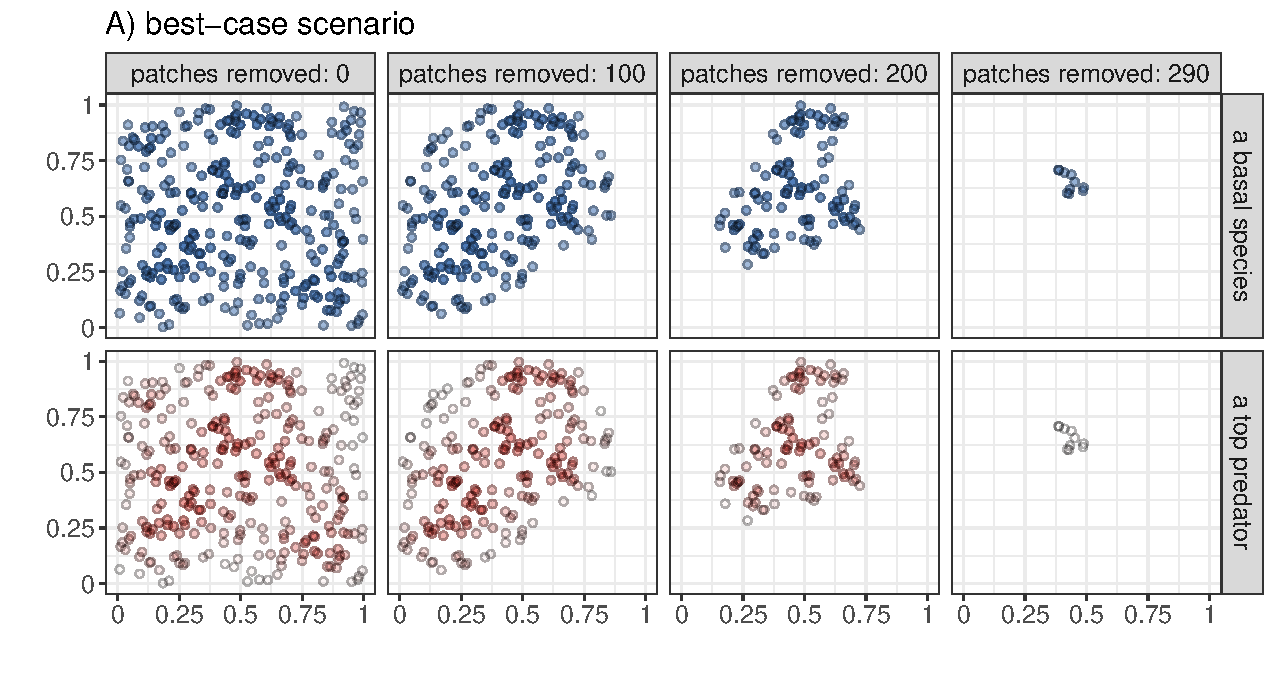
\includegraphics[width=0.83\textwidth]{best-case_scenario.pdf}
  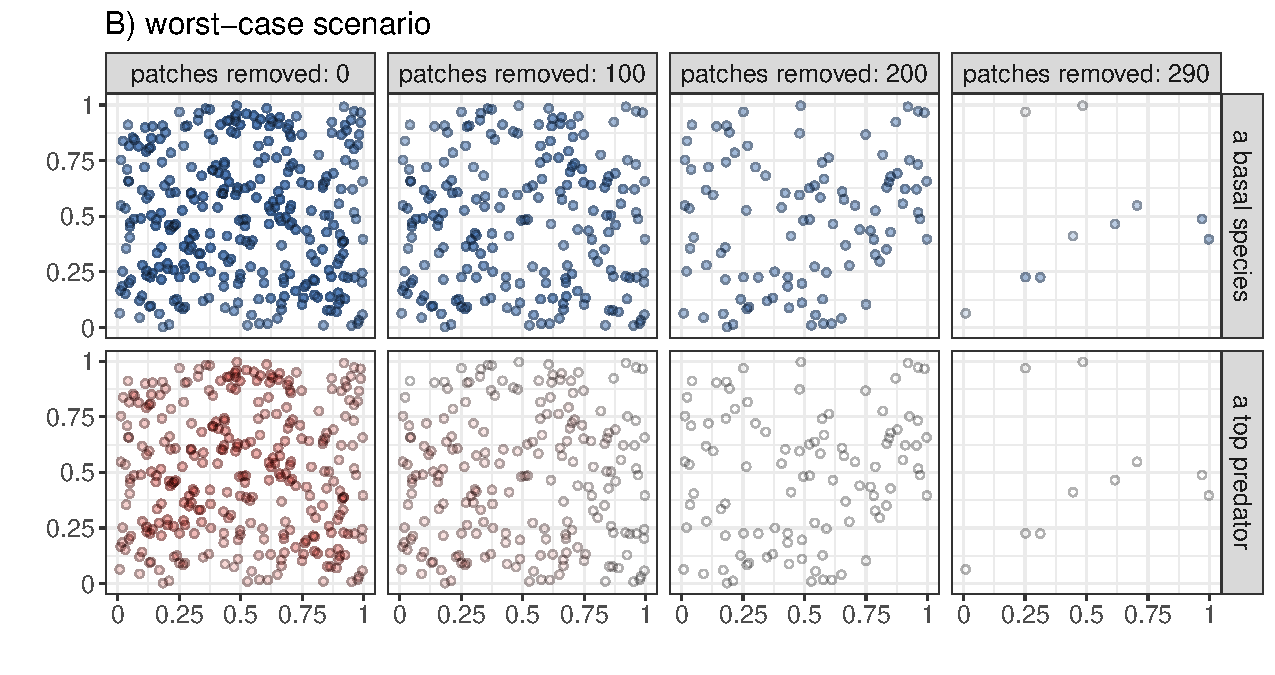
\includegraphics[width=0.83\textwidth]{worst-case_scenario.pdf}
  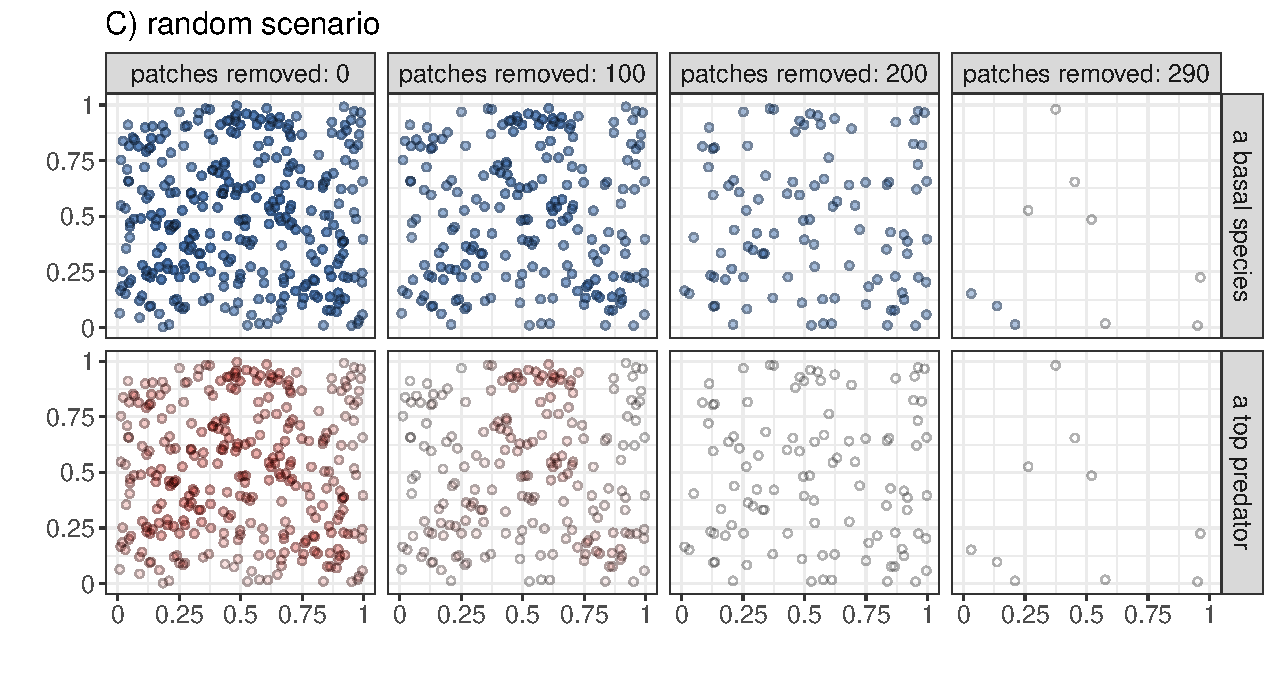
\includegraphics[width=0.83\textwidth]{random_scenario.pdf}
  \caption{Patch occupancies along a habitat loss gradient, for a basal species (blue) and a top predator (red) in a model food web with 300 consumer and 100 basal species. Axes are coordinates of the landscape, circles are patches, and their shading is proportional to local persistence probabilities (dark blue/red: $100\%$ persistence; empty circle: $0\%$). In the best-case scenario (A), we first remove patches that contribute the least to the metapopulation capacity of the basal species; in the worst-case scenario (B), we start with patches that contribute the most; and in (C) we remove patches randomly. The dispersal distance $\xi_i$ is $0.055$ for all species, and baseline extinction probabilities $\pi_i$ increase linearly with trophic level.}
  \label{fig:loss_example}
\end{figure}


\clearpage

\begin{figure}
  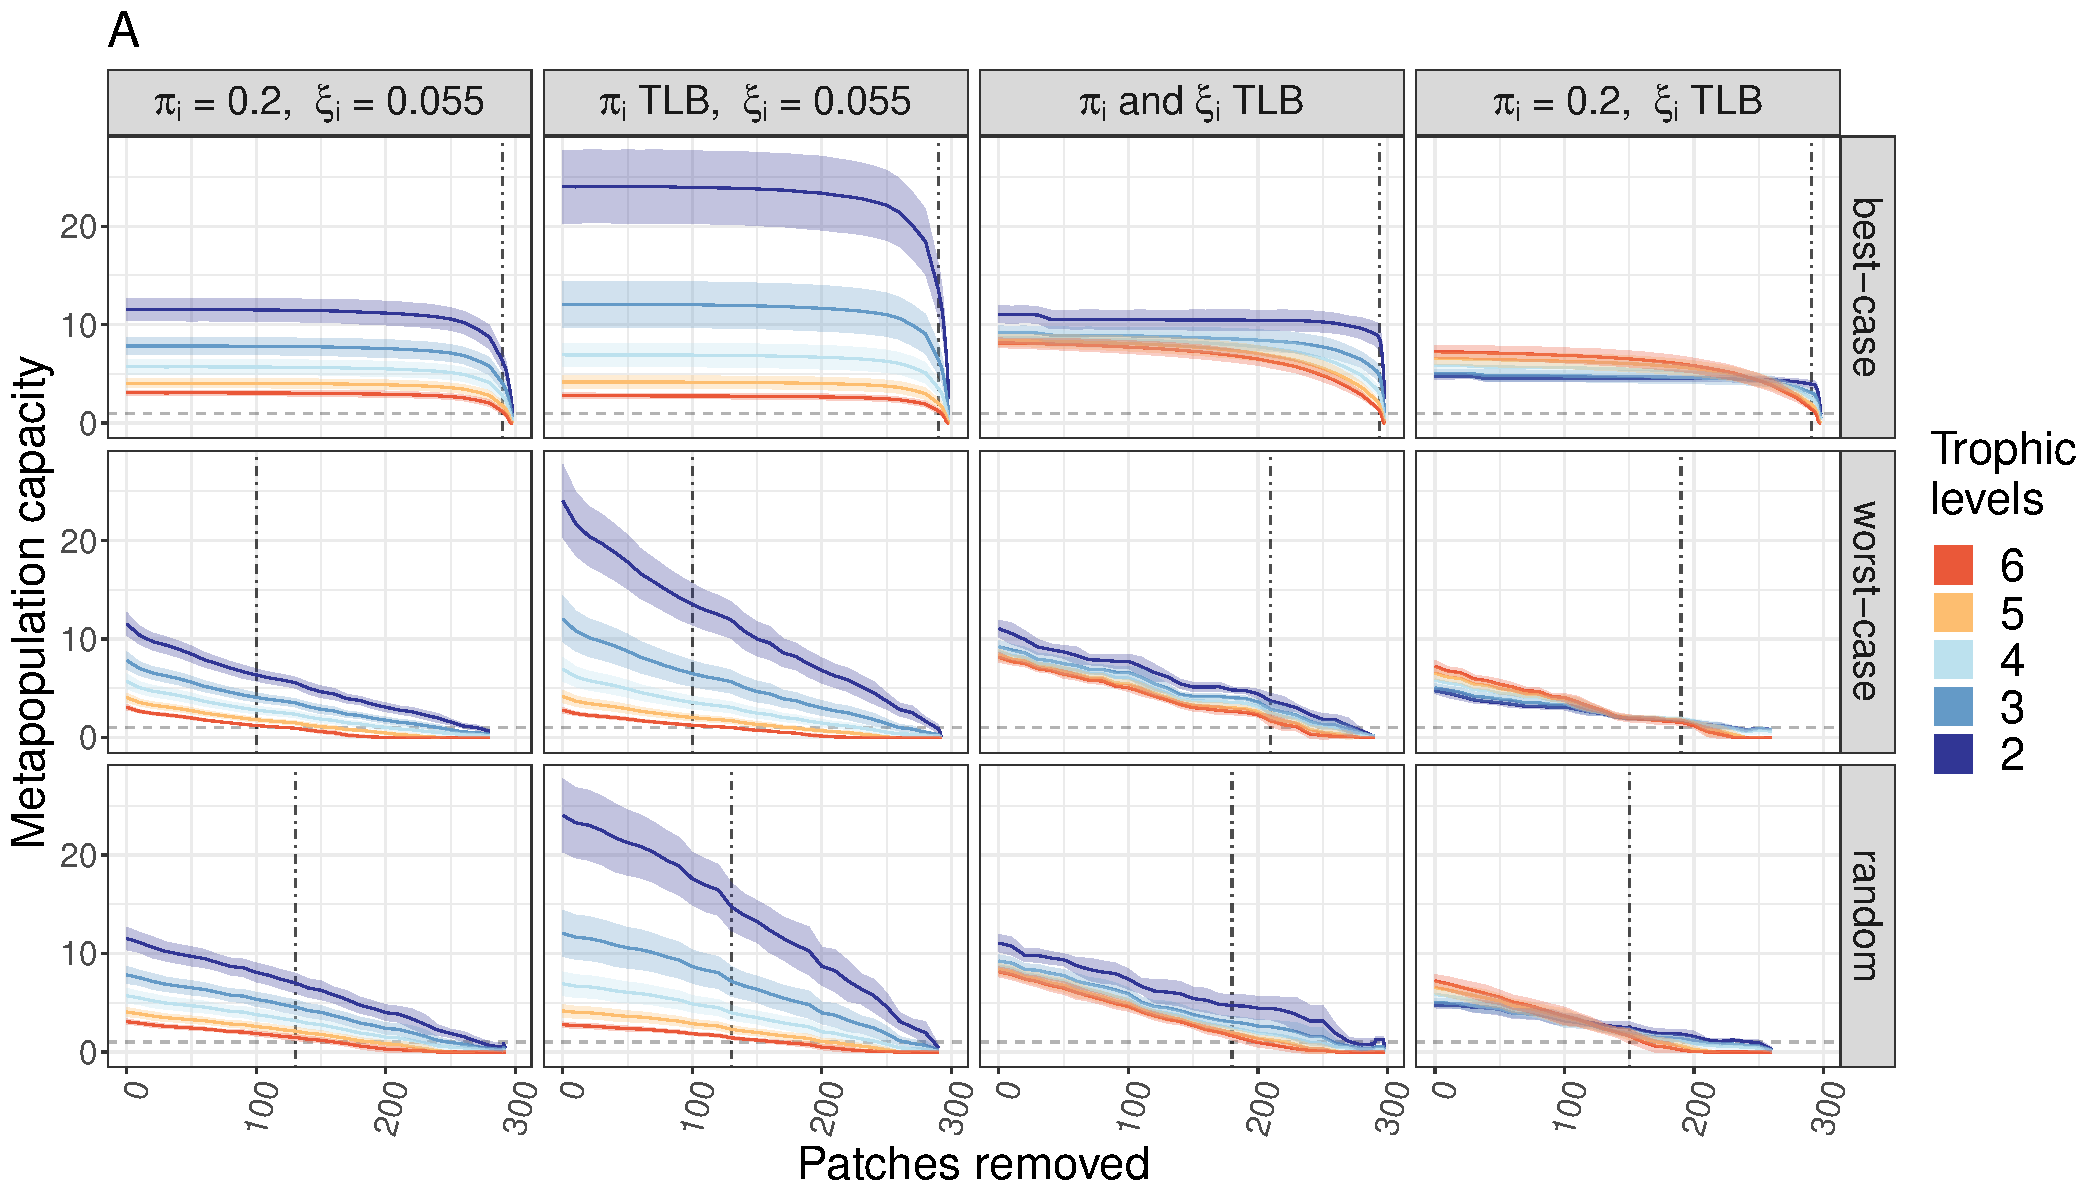
\includegraphics[width=0.8\textwidth,valign=t]{lambda_Model_food_web_with_300_consumer_and_100_basal_species_basal_1_1.pdf}
  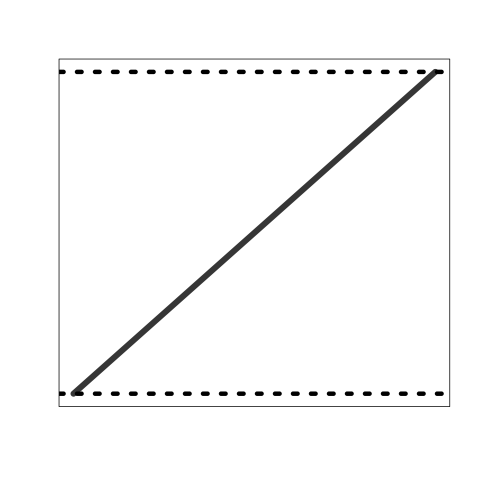
\includegraphics[width=0.19\textwidth,valign=t]{fform_1_1.png}
  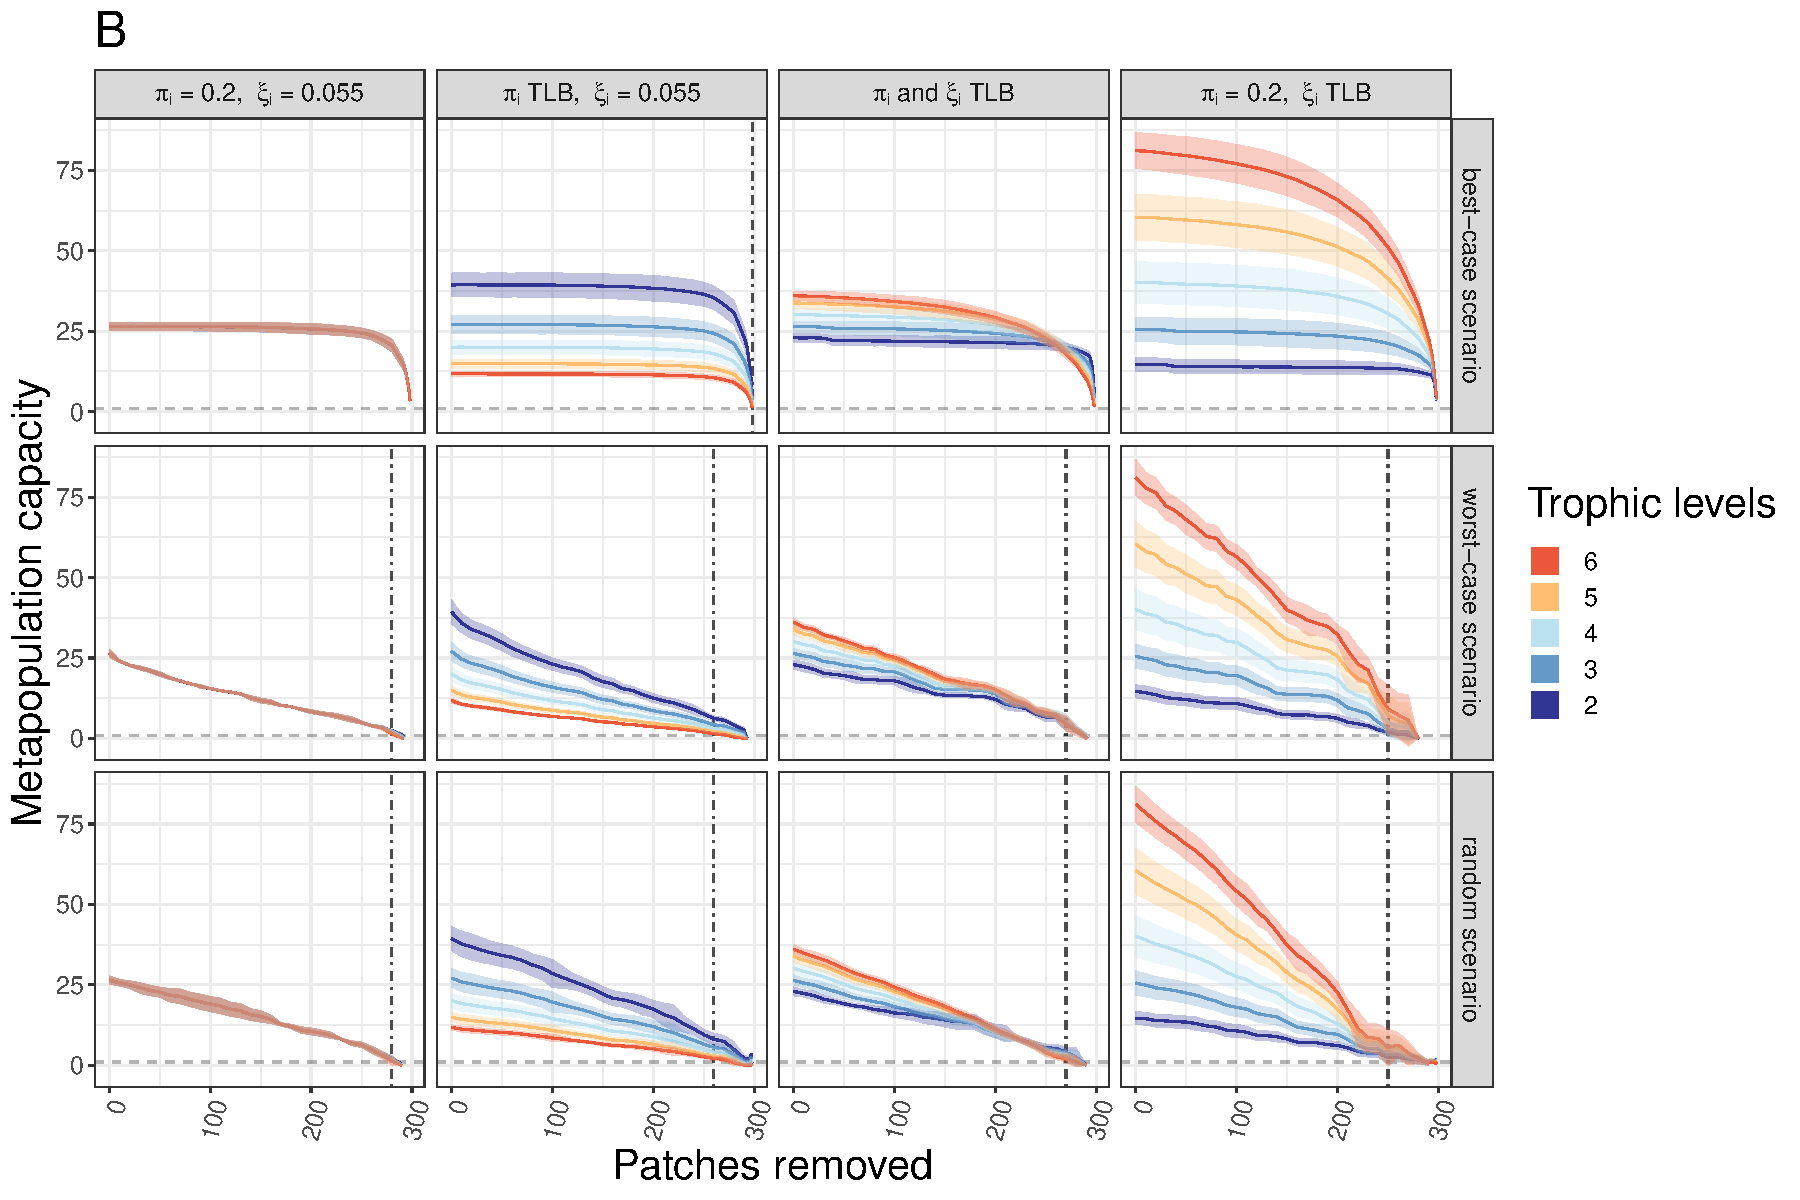
\includegraphics[width=0.8\textwidth,valign=t]{lambda_Model_food_web_with_300_consumer_and_100_basal_species_basal_5_1.pdf}
    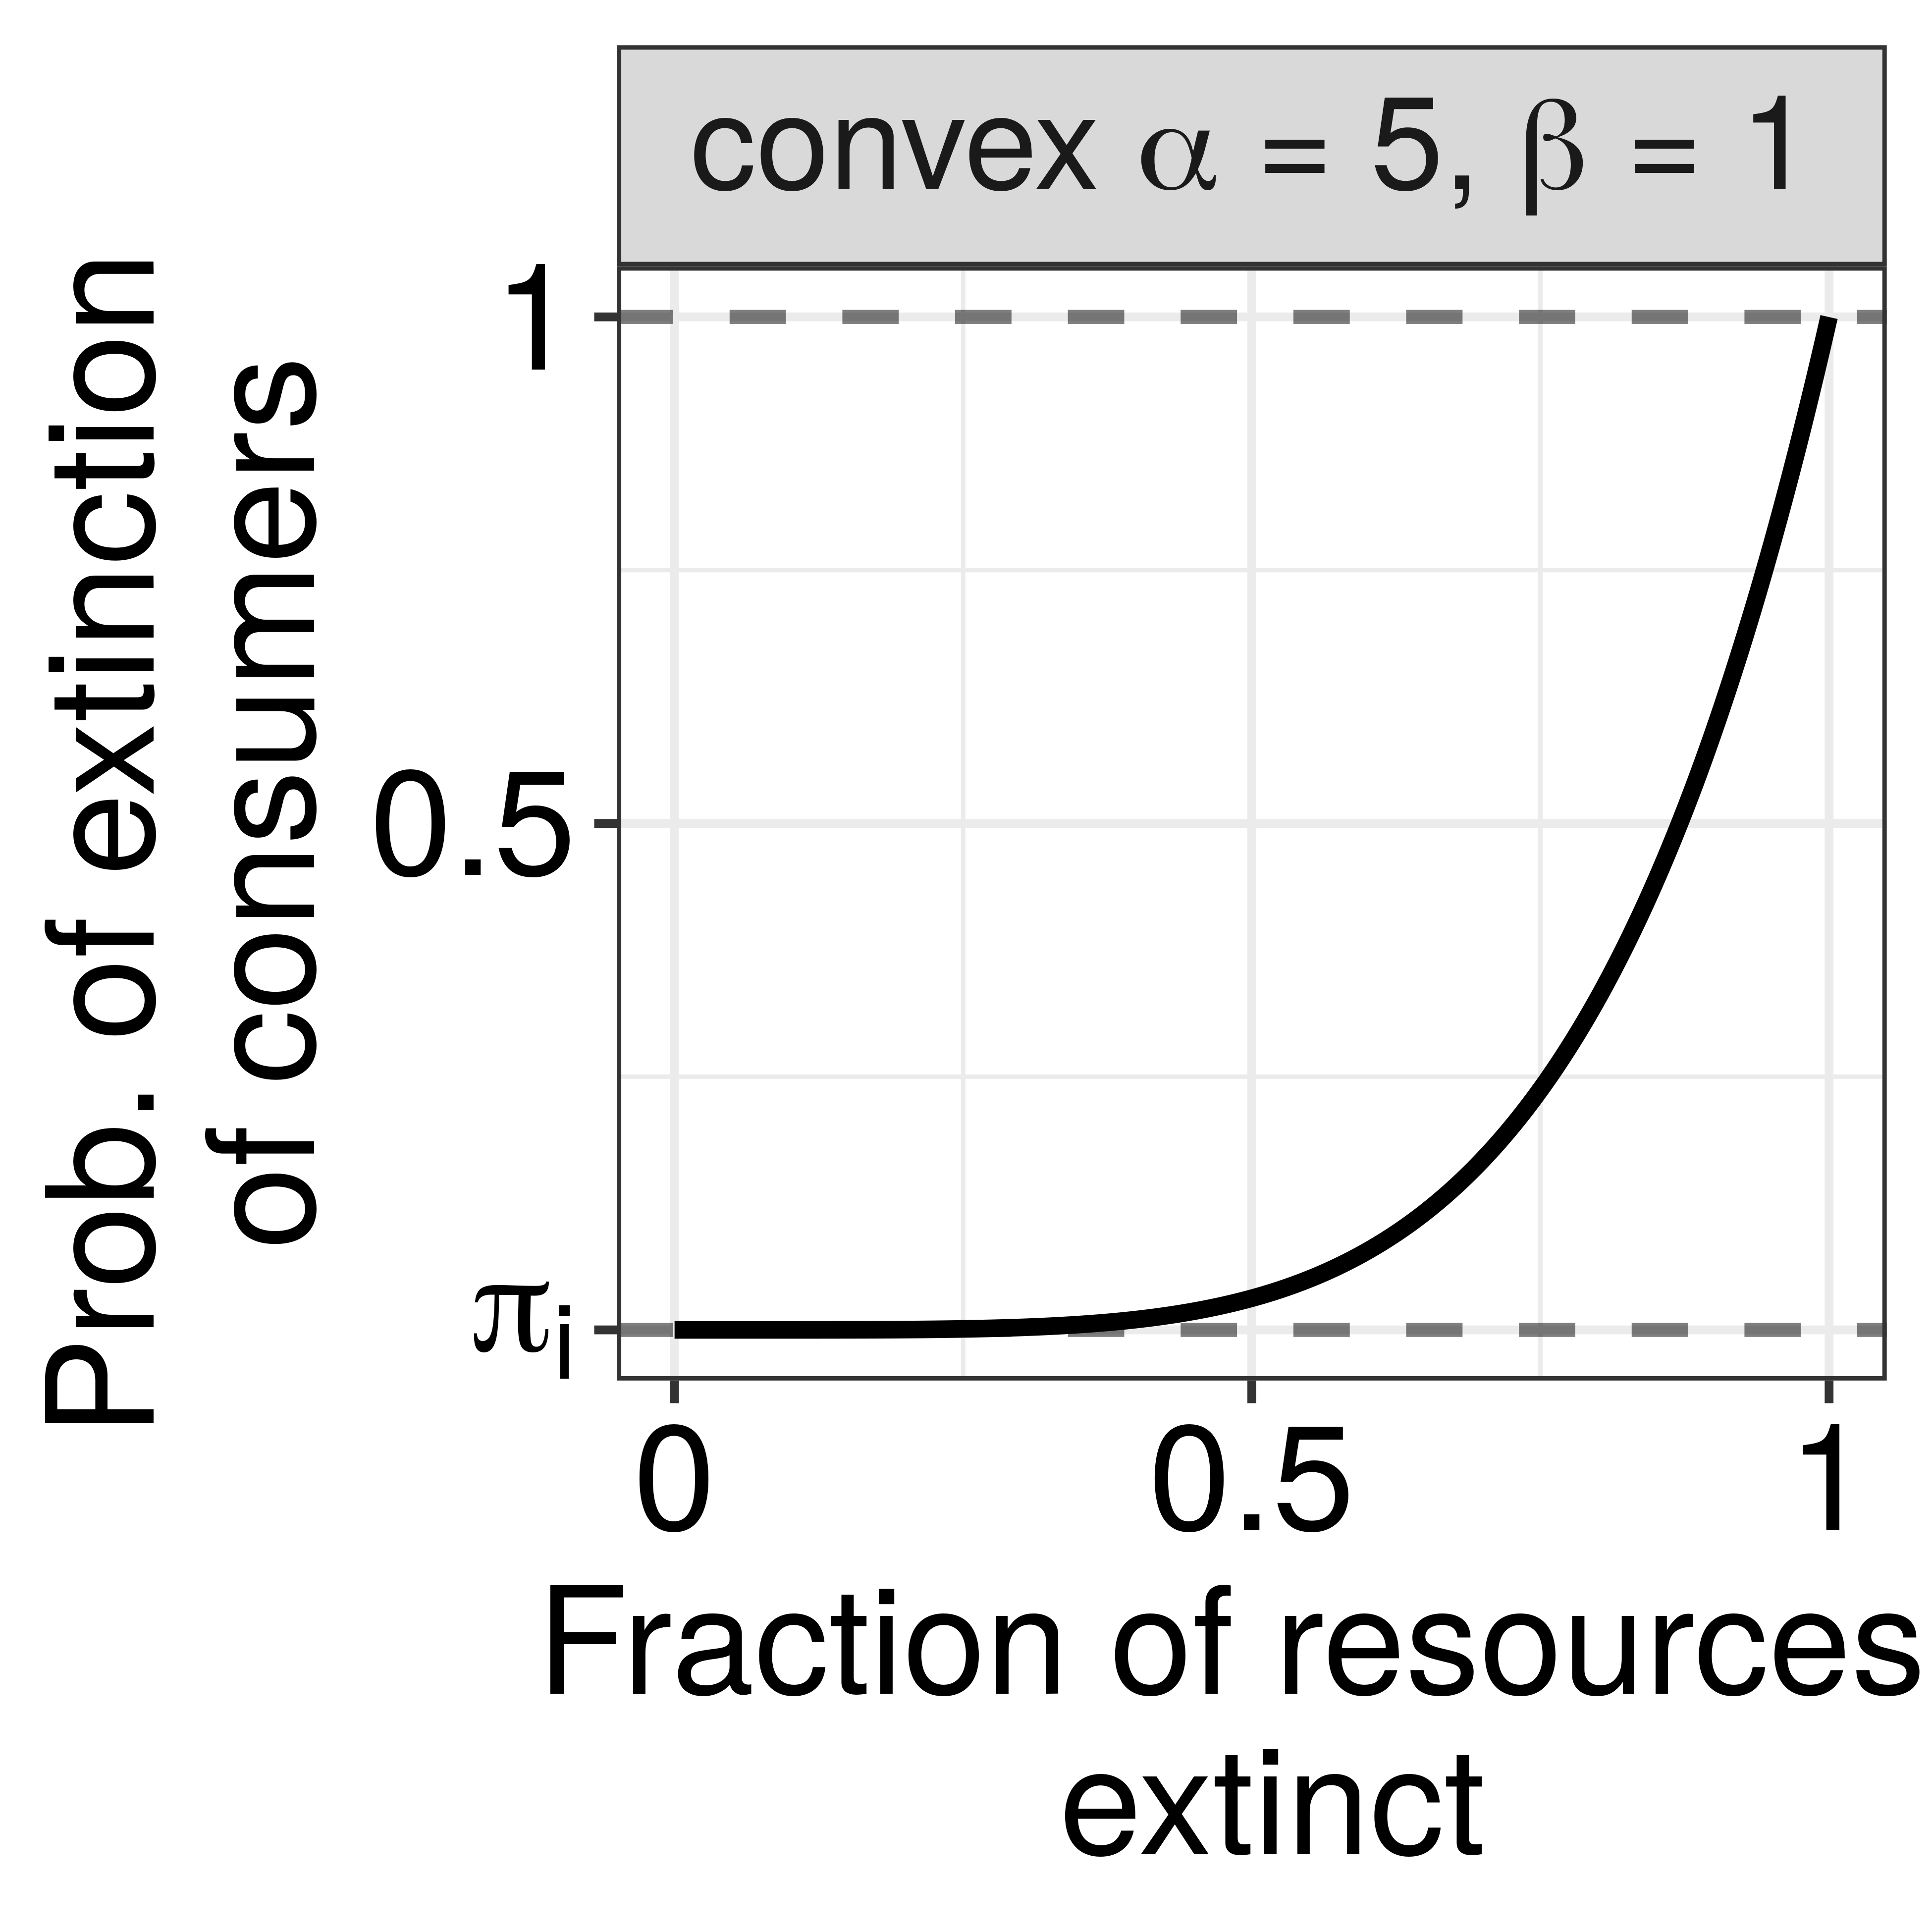
\includegraphics[width=0.19\textwidth,valign=t]{fform_5_1.png}
  \caption{Effect of habitat loss on species persistence in a model food web with 300 consumer and 100 basal species. A-D are for different functional forms of a consumer's response to the loss of resources (top right insets). Species are grouped into trophic levels (color legends); lines show the mean and the bands around them the one standard deviation range of the metapopulation capacities of species in the corresponding trophic level. Rows indicate patch-removal scenario (best-case, worst-case, and random); columns the parameterization method: baseline extinction probabilities $\pi_i$ and dispersal distances $\xi_i$ can either take on one value across all species, or increase with trophic level (trophic level-based, TLB). Horizontal dashed lines highlight a metapopulation capacity of $1$, the threshold for long-term species persistence. Vertical dashed lines show when the metapopulation capacity of the top species in the food web drops below this threshold.}
  \label{fig:patchloss}
\end{figure}

\begin{figure}\ContinuedFloat
  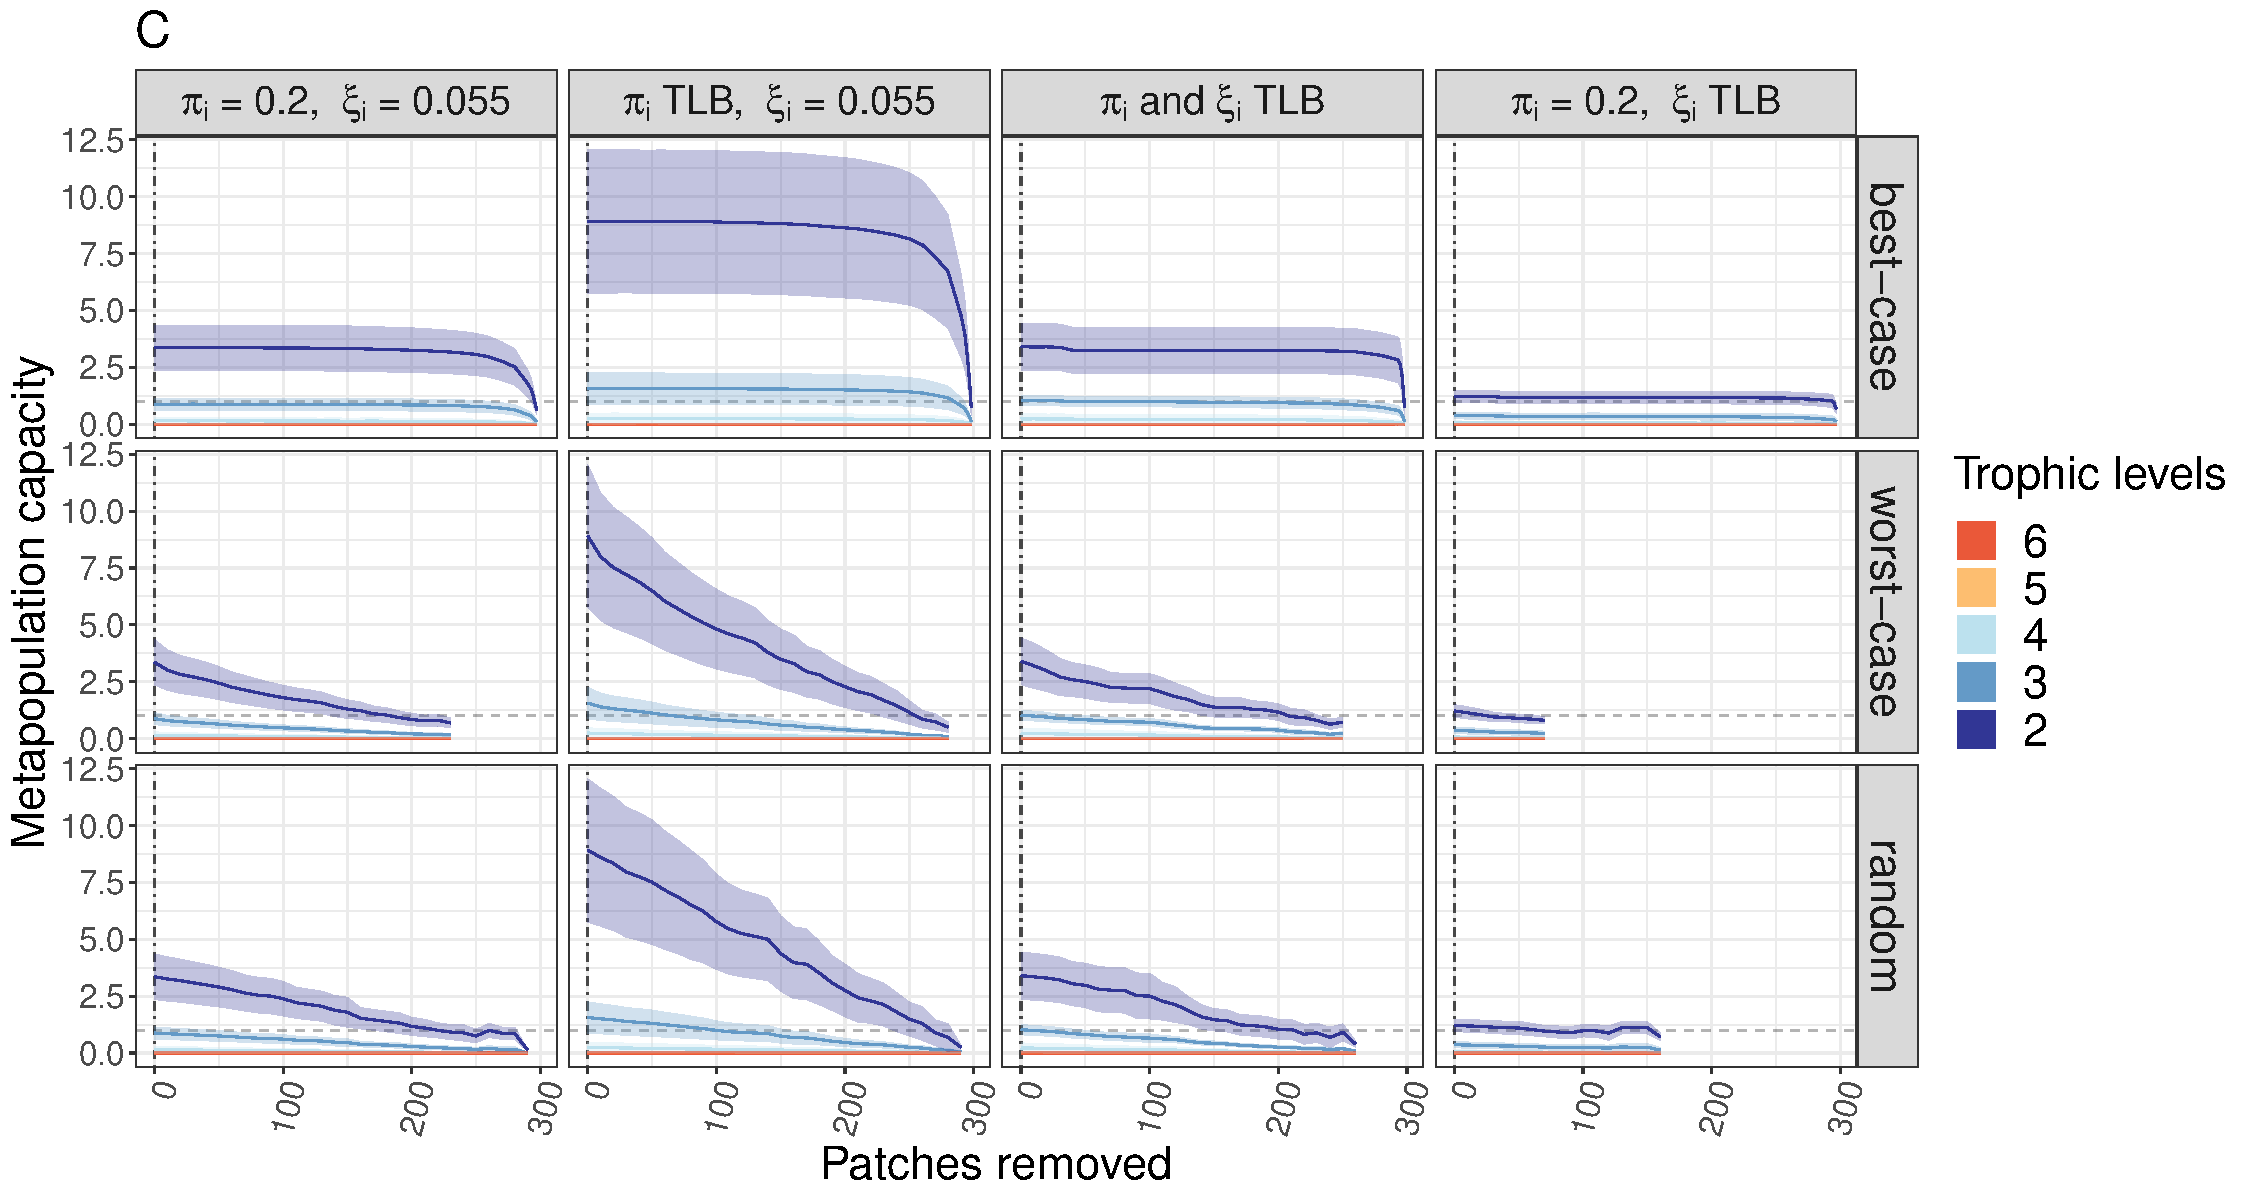
\includegraphics[width=0.8\textwidth,valign=t]{lambda_Model_food_web_with_300_consumer_and_100_basal_species_basal_1_5.pdf}
  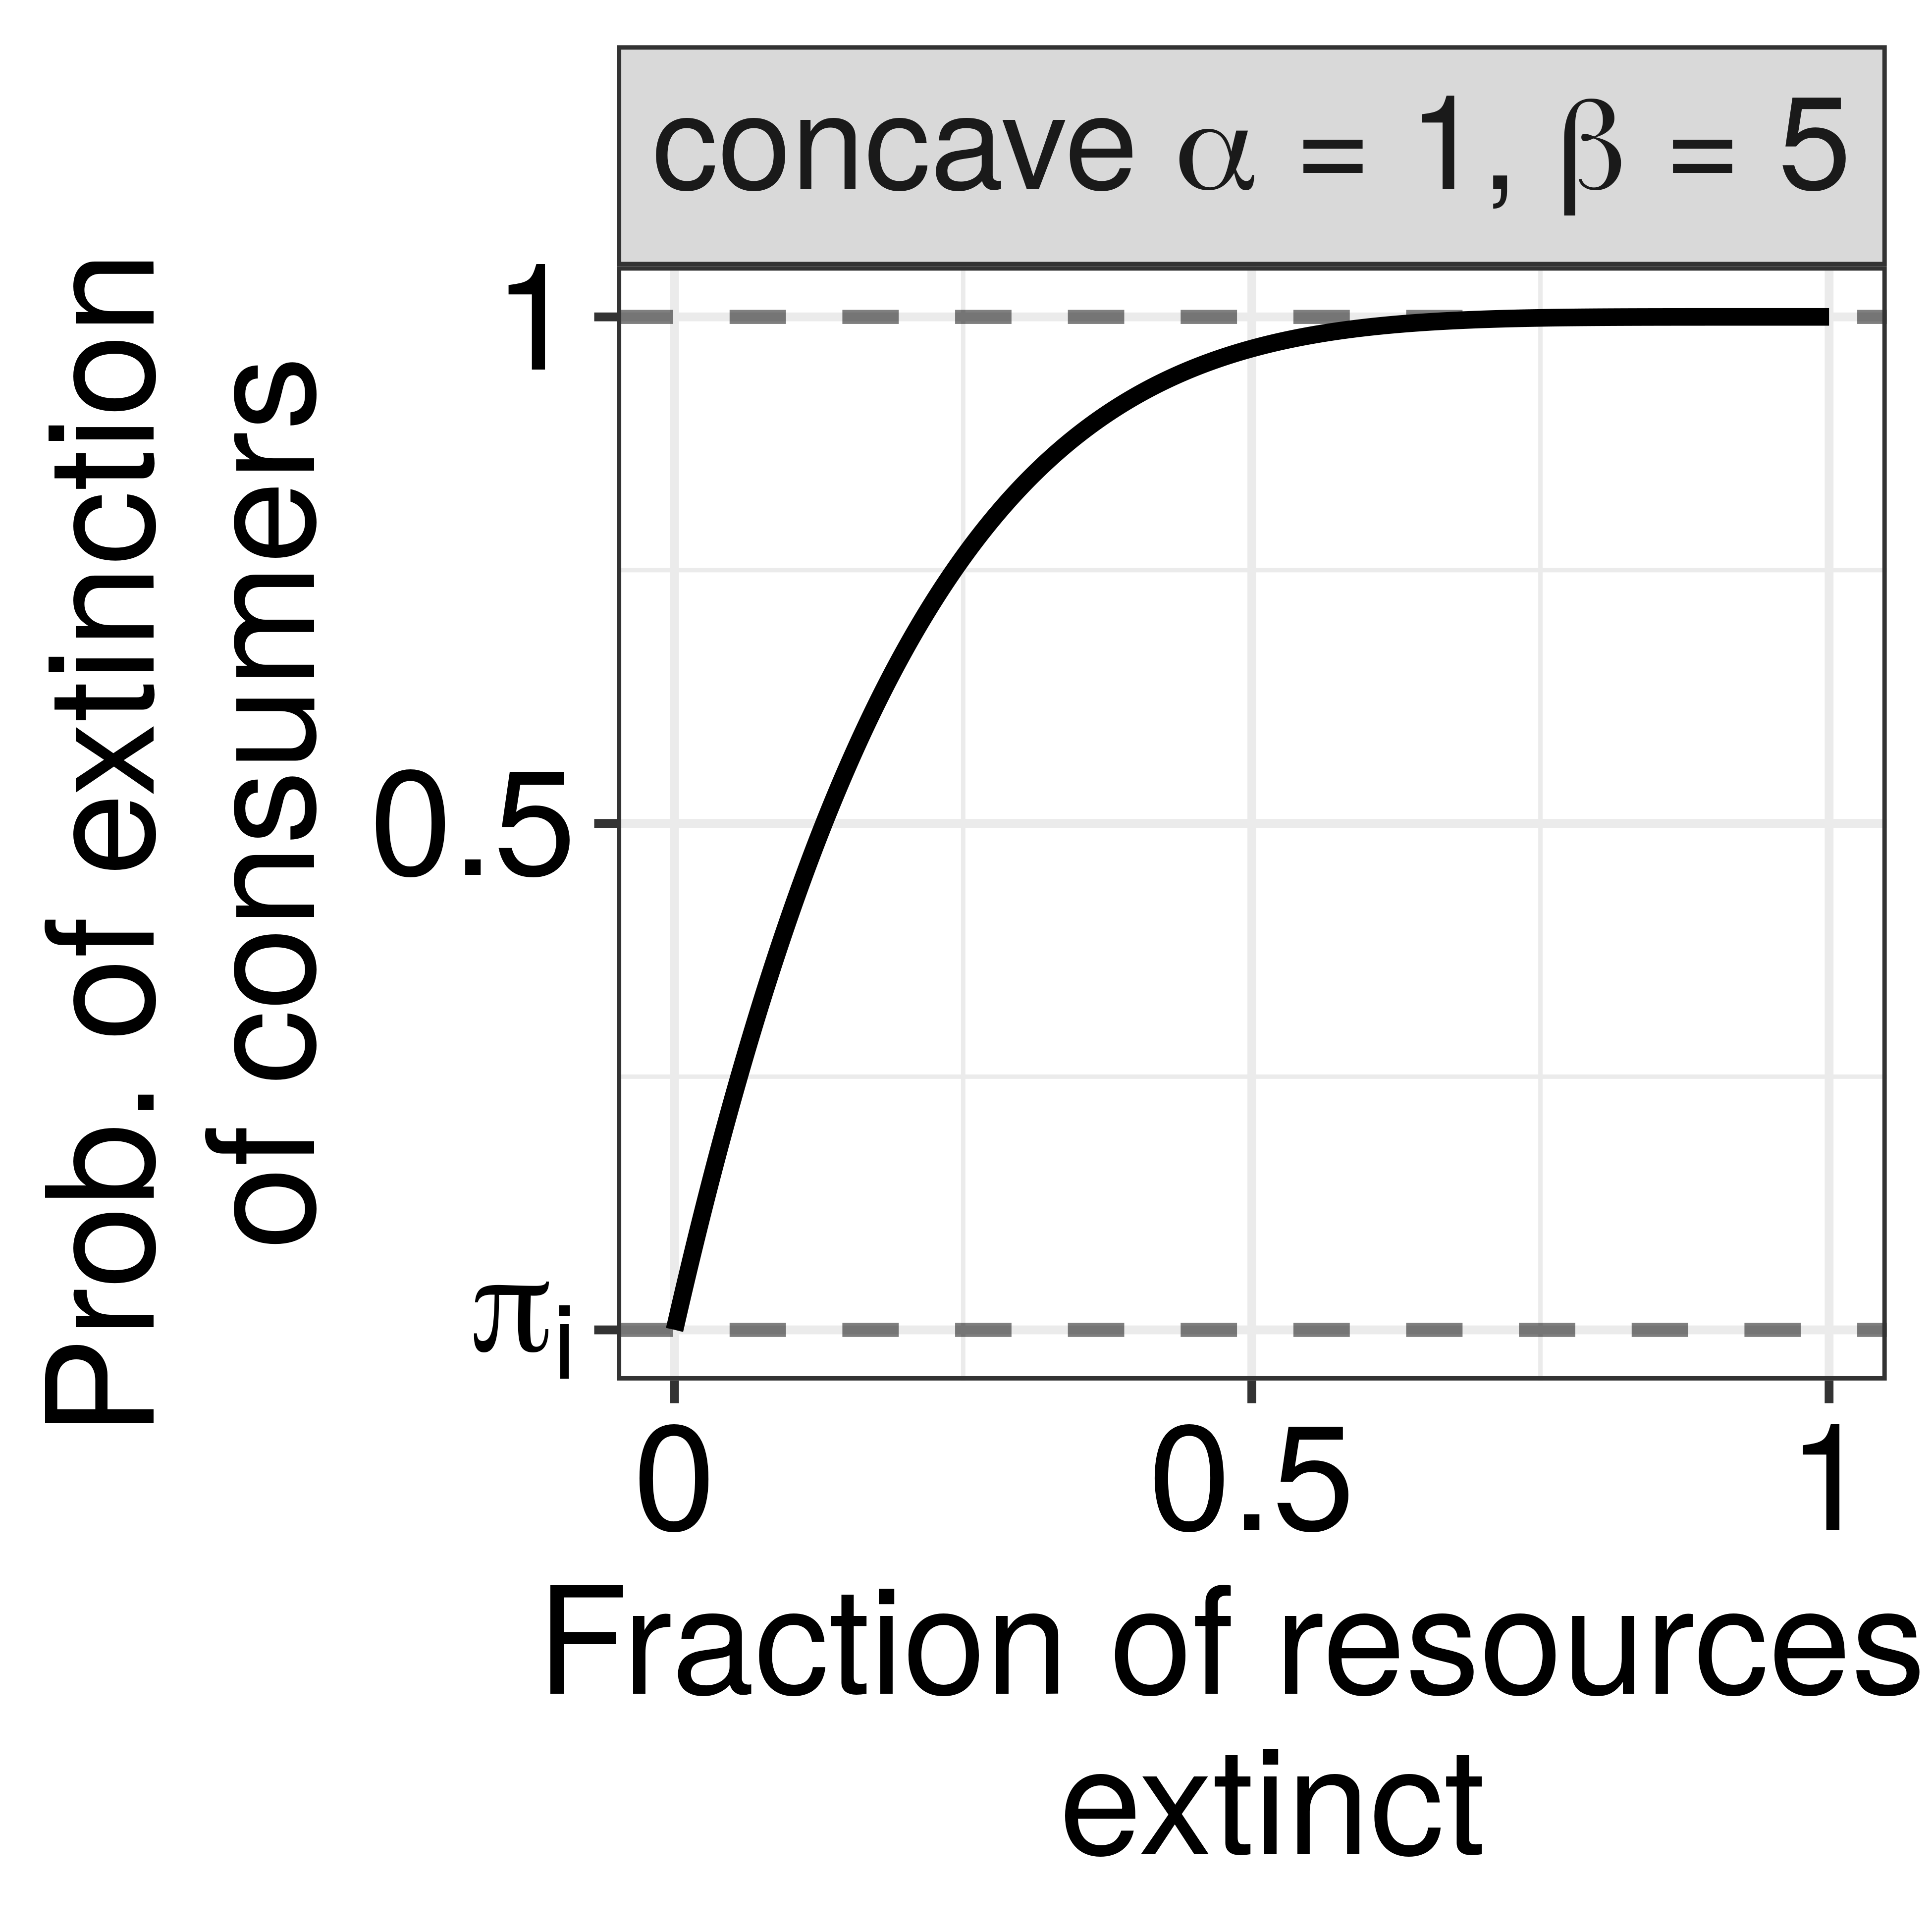
\includegraphics[width=0.19\textwidth,valign=t]{fform_1_5.png}
  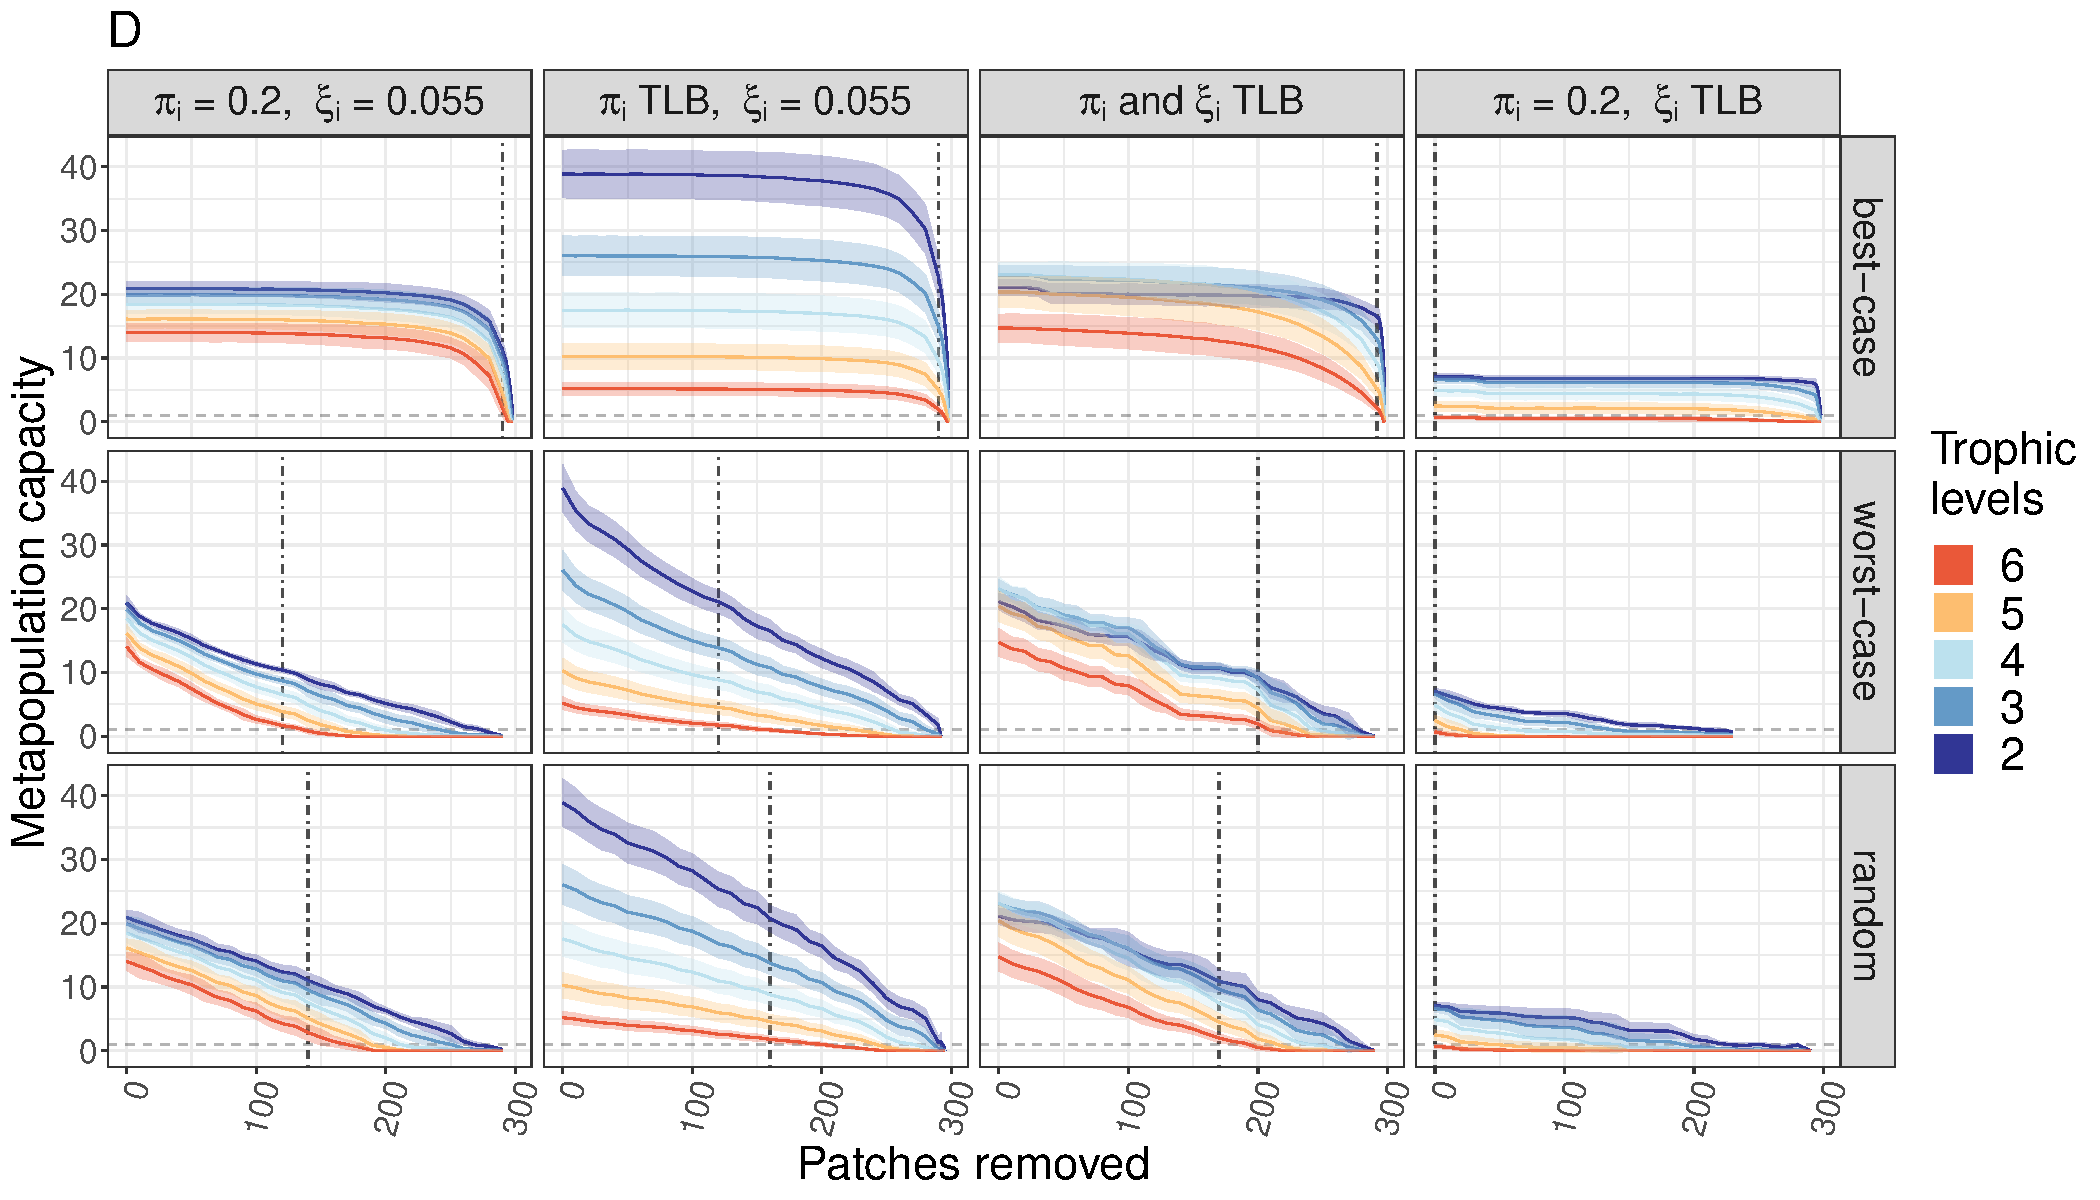
\includegraphics[width=0.8\textwidth,valign=t]{lambda_Model_food_web_with_300_consumer_and_100_basal_species_basal_5_5.pdf}
    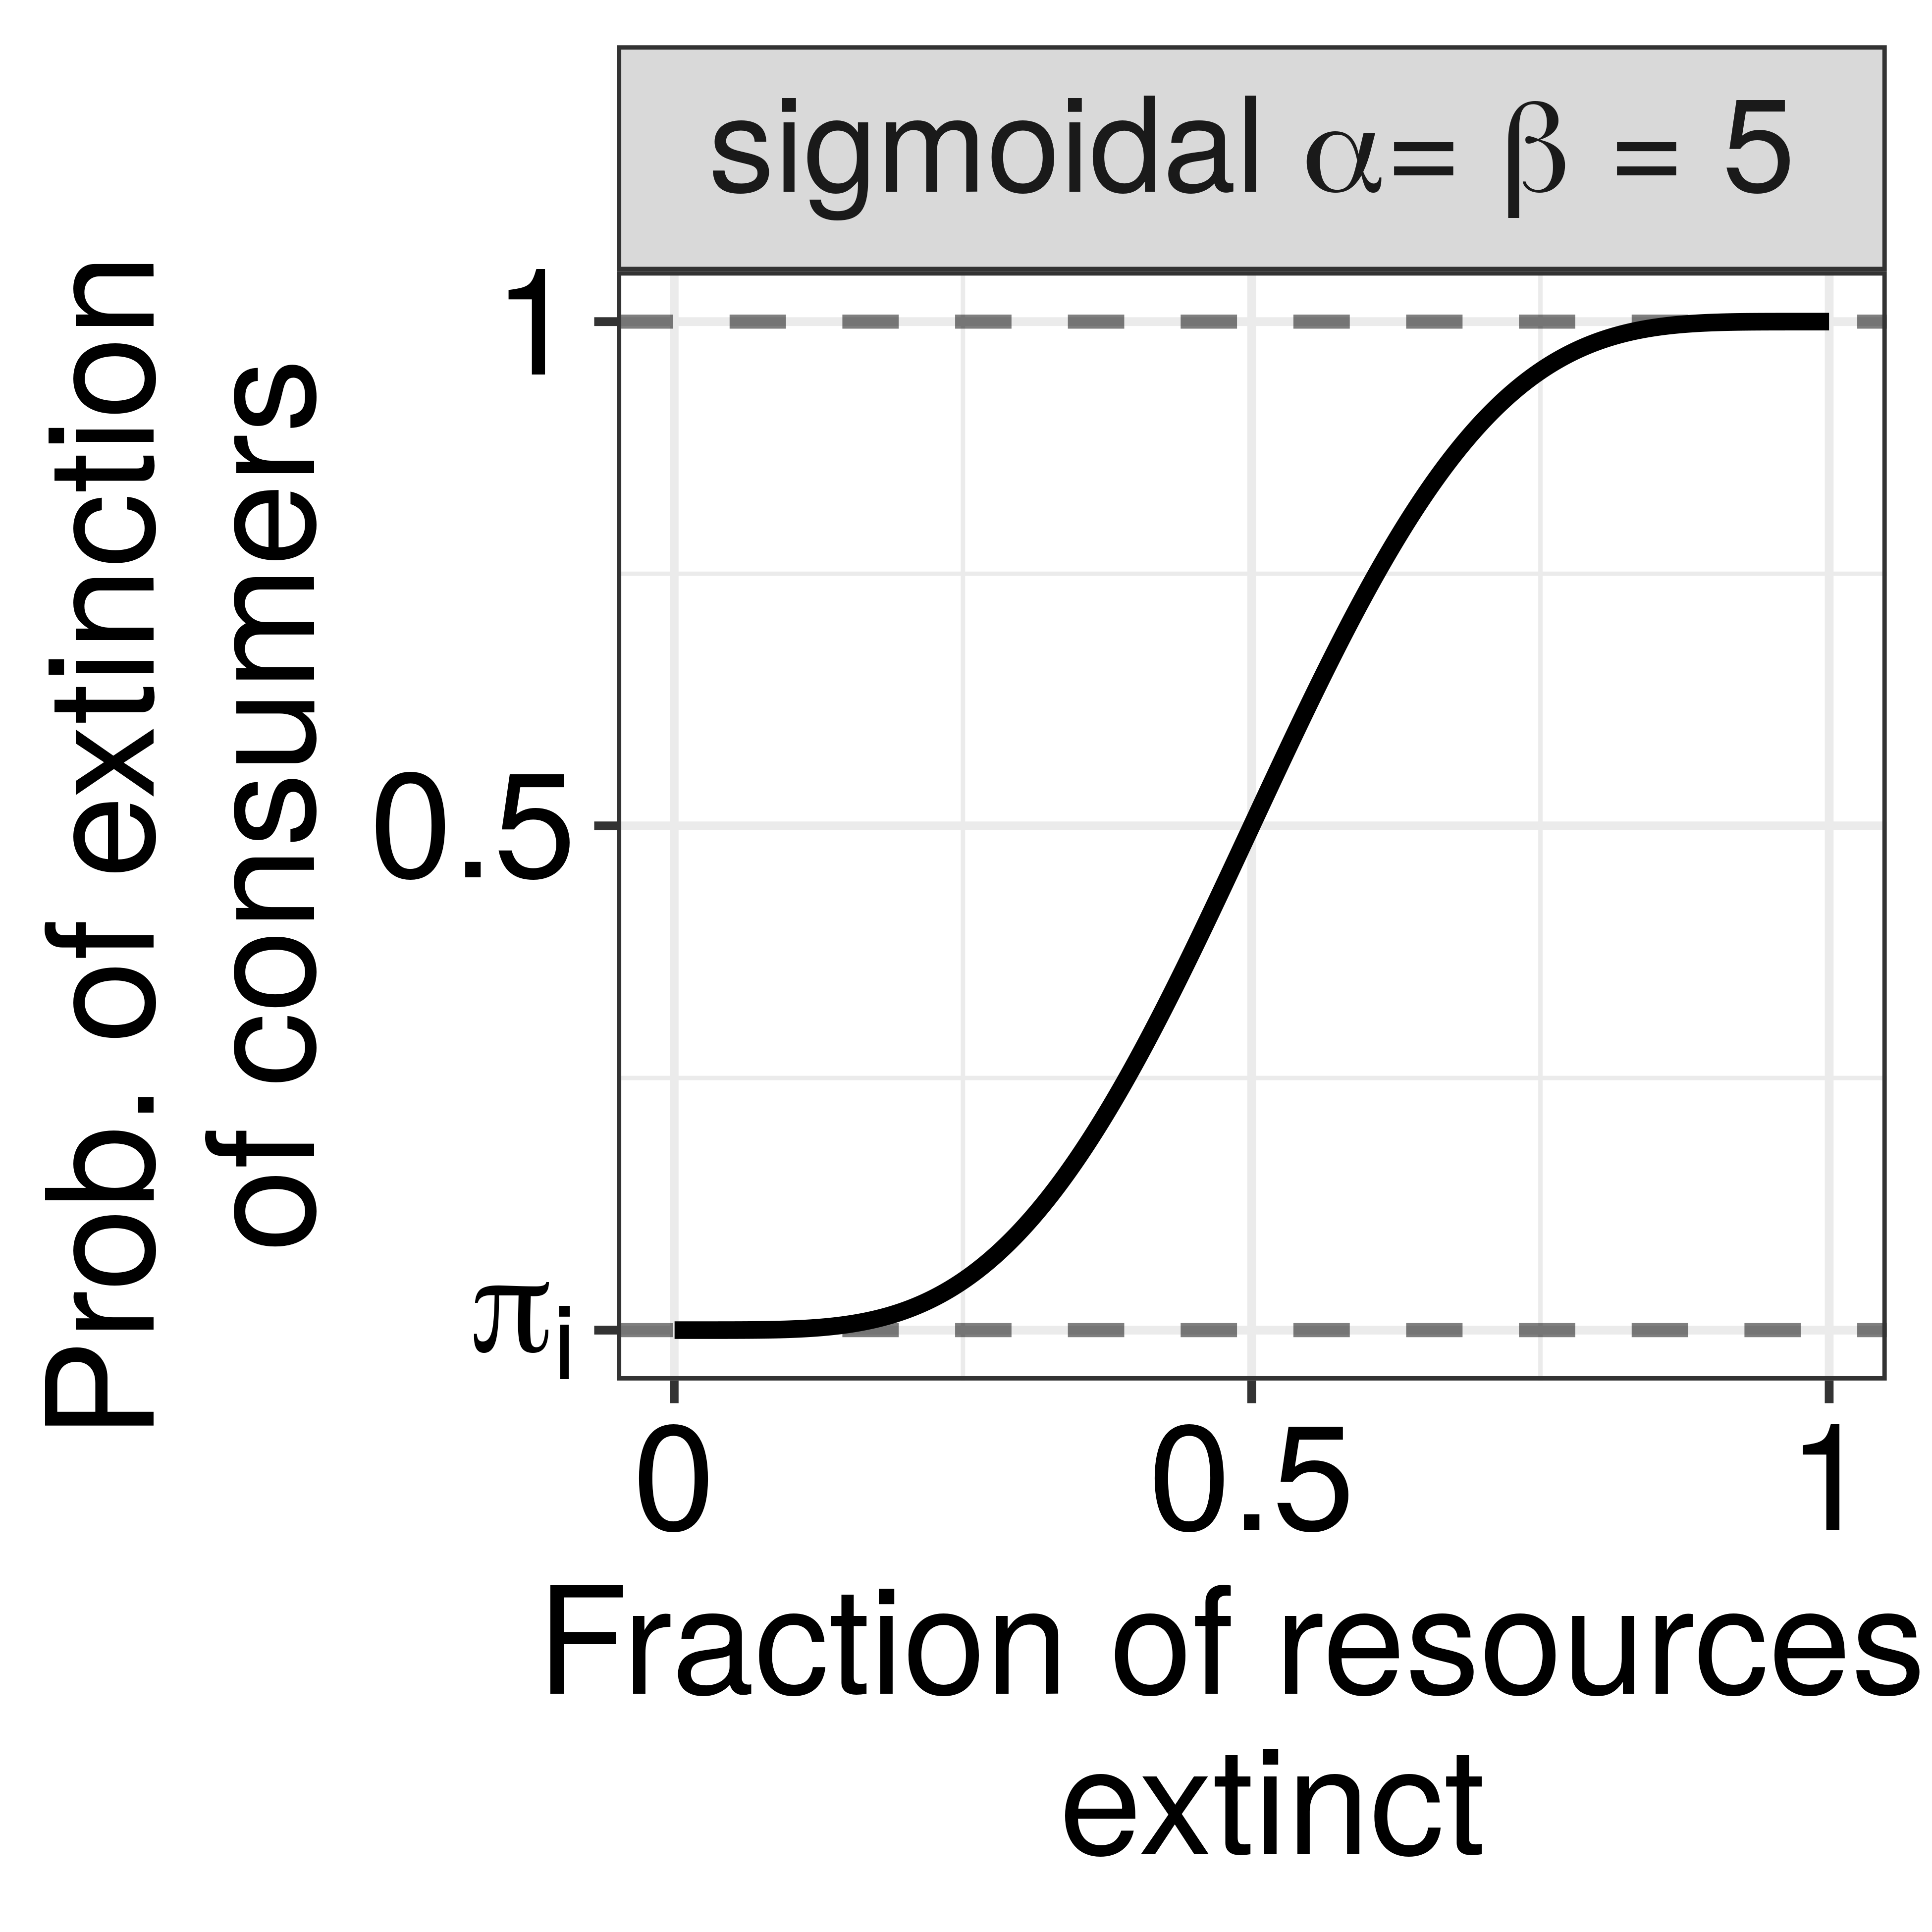
\includegraphics[width=0.19\textwidth,valign=t]{fform_5_5.png}
  \caption{Figure continued.}
  \label{fig:patchloss_2}
\end{figure}

\clearpage


\begin{figure}[!p]
  \centering
  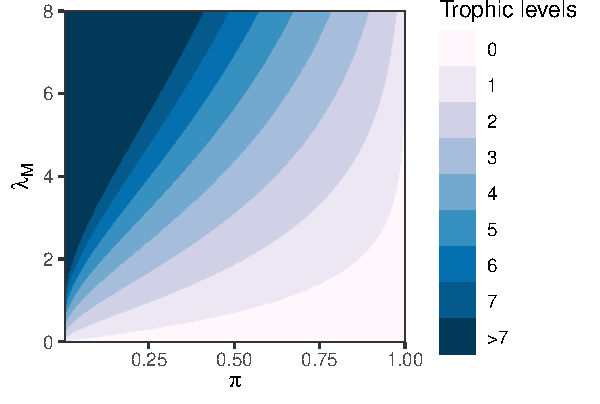
\includegraphics[width=0.65\textwidth]{TL_chain.pdf}
  \caption{The maximum number of trophic levels in trophic chain metacommunities, as a function of a common baseline extinction probability $\pi$ and the leading eigenvalue of a common landscape matrix $\lambda_M$. Unless $\pi$ is low and $\lambda_M$ simultaneously high, the metacommunity structure itself puts a cap on the number of possible trophic levels. This color map was generated by iterating Eq.~\ref{eq:chain} until metapopulation capacities dropped below the persistence threshold of $1$. However, the same result obtains by approximating the maximum number of trophic levels simply with $-\lambda_M\log(\pi)$ (Eq.~\ref{eq:Tapprox}; see also \SI, Figure~\ref{SI:fig:TL_compare}).}
  \label{fig:TL_chain}
\end{figure}


\clearpage


\begin{figure}
  \indent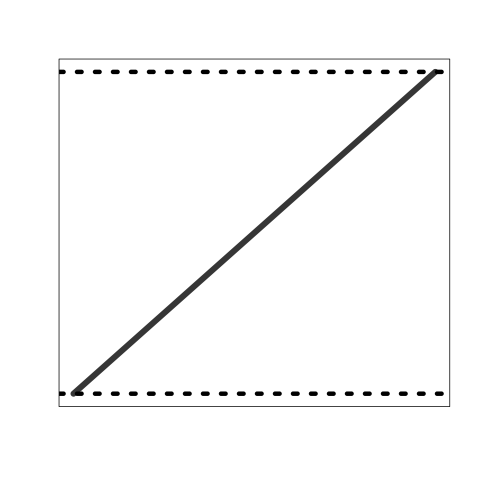
\includegraphics[width=0.18\textwidth]{fform_1_1.png}
  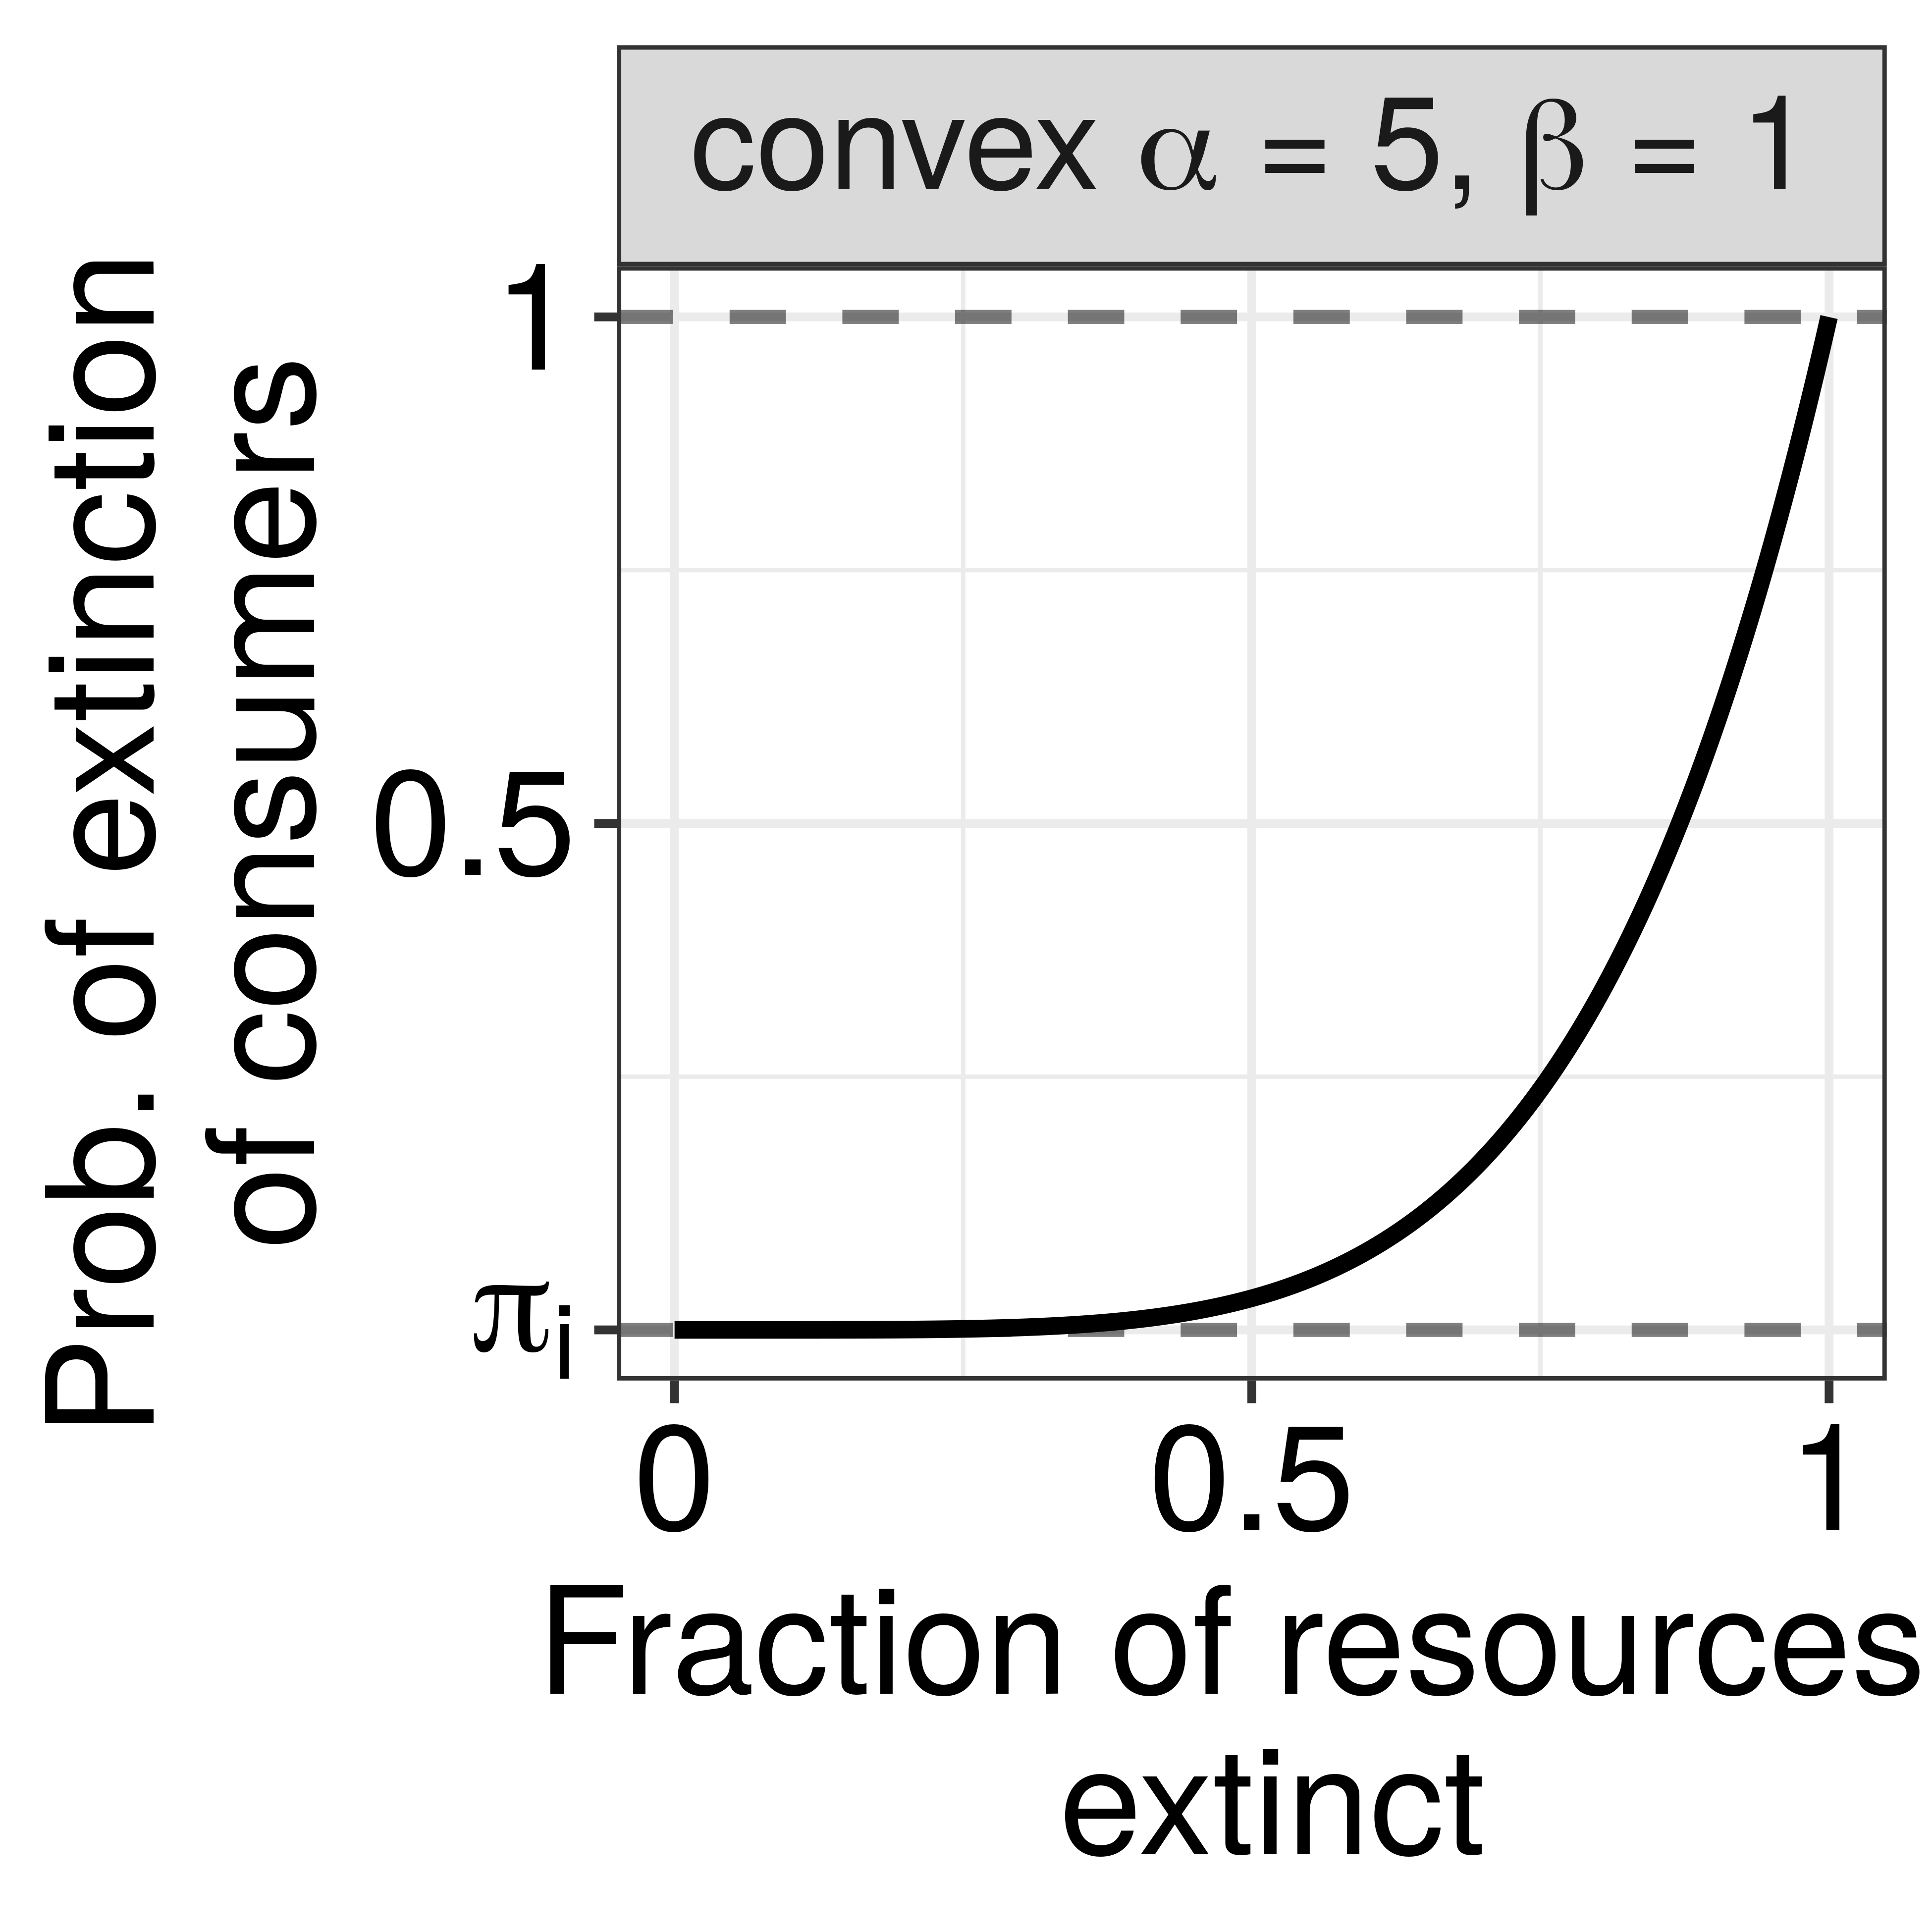
\includegraphics[width=0.18\textwidth]{fform_5_1.png}
  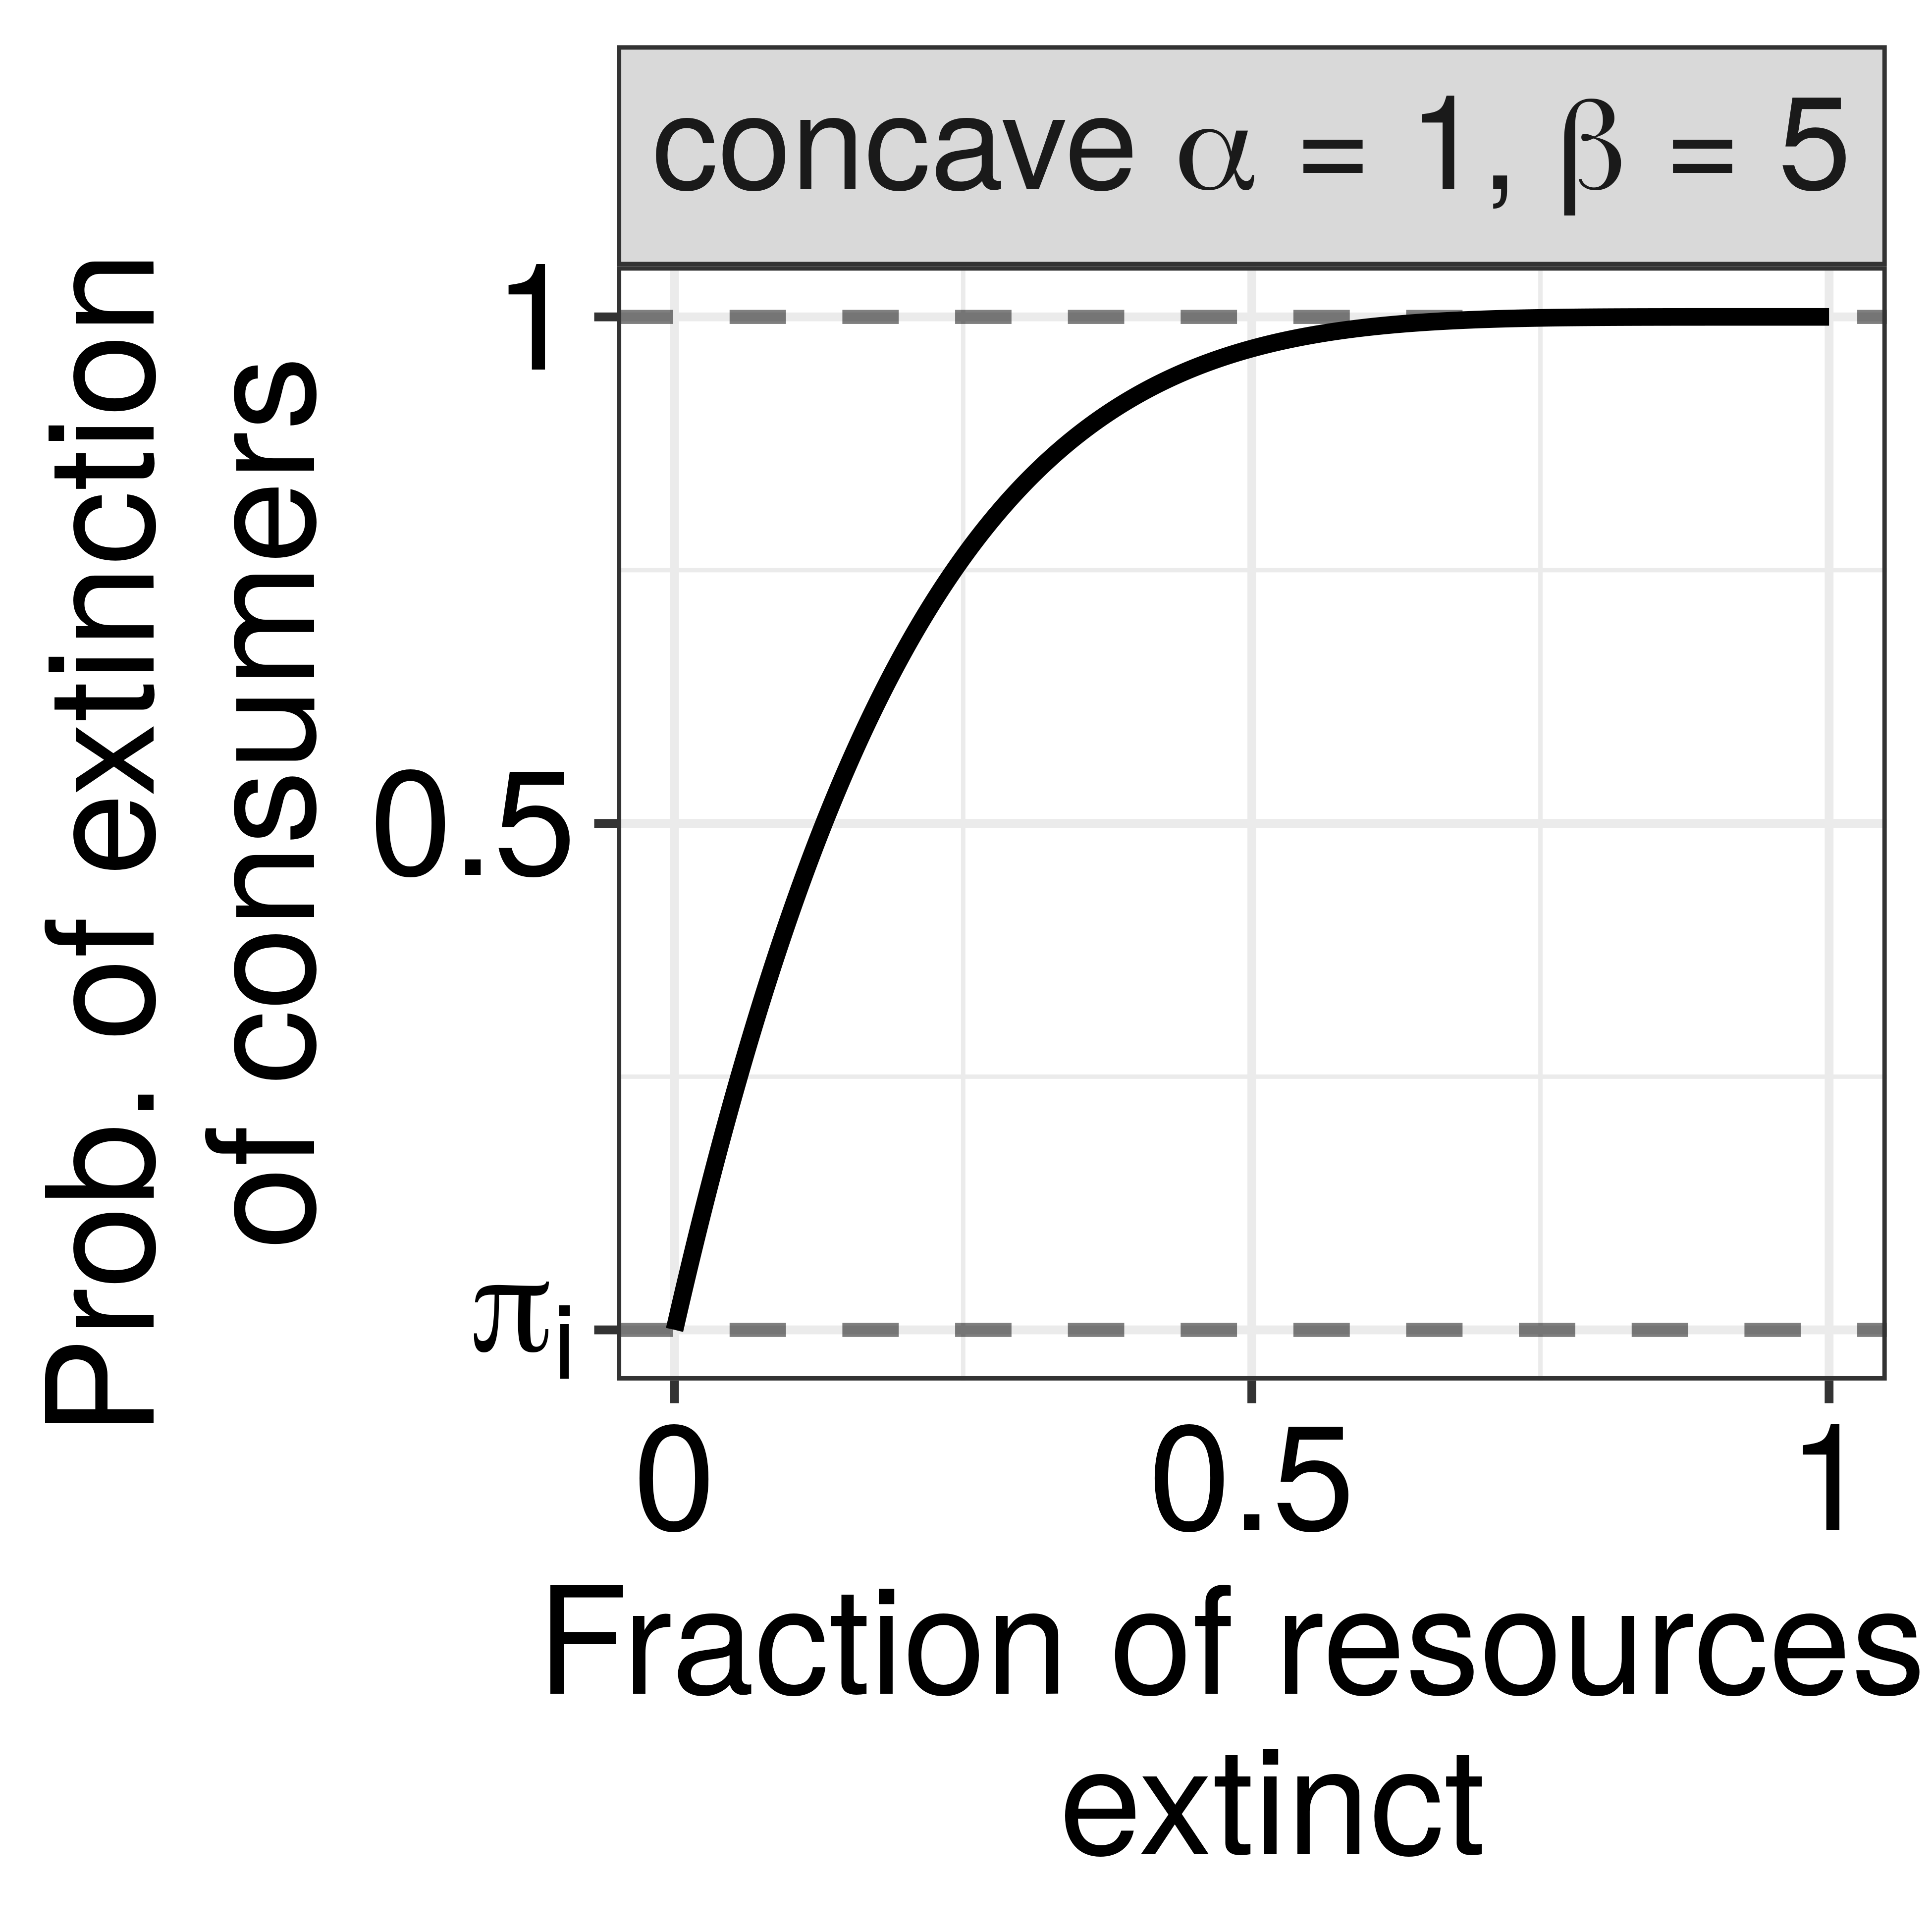
\includegraphics[width=0.18\textwidth]{fform_1_5.png}
  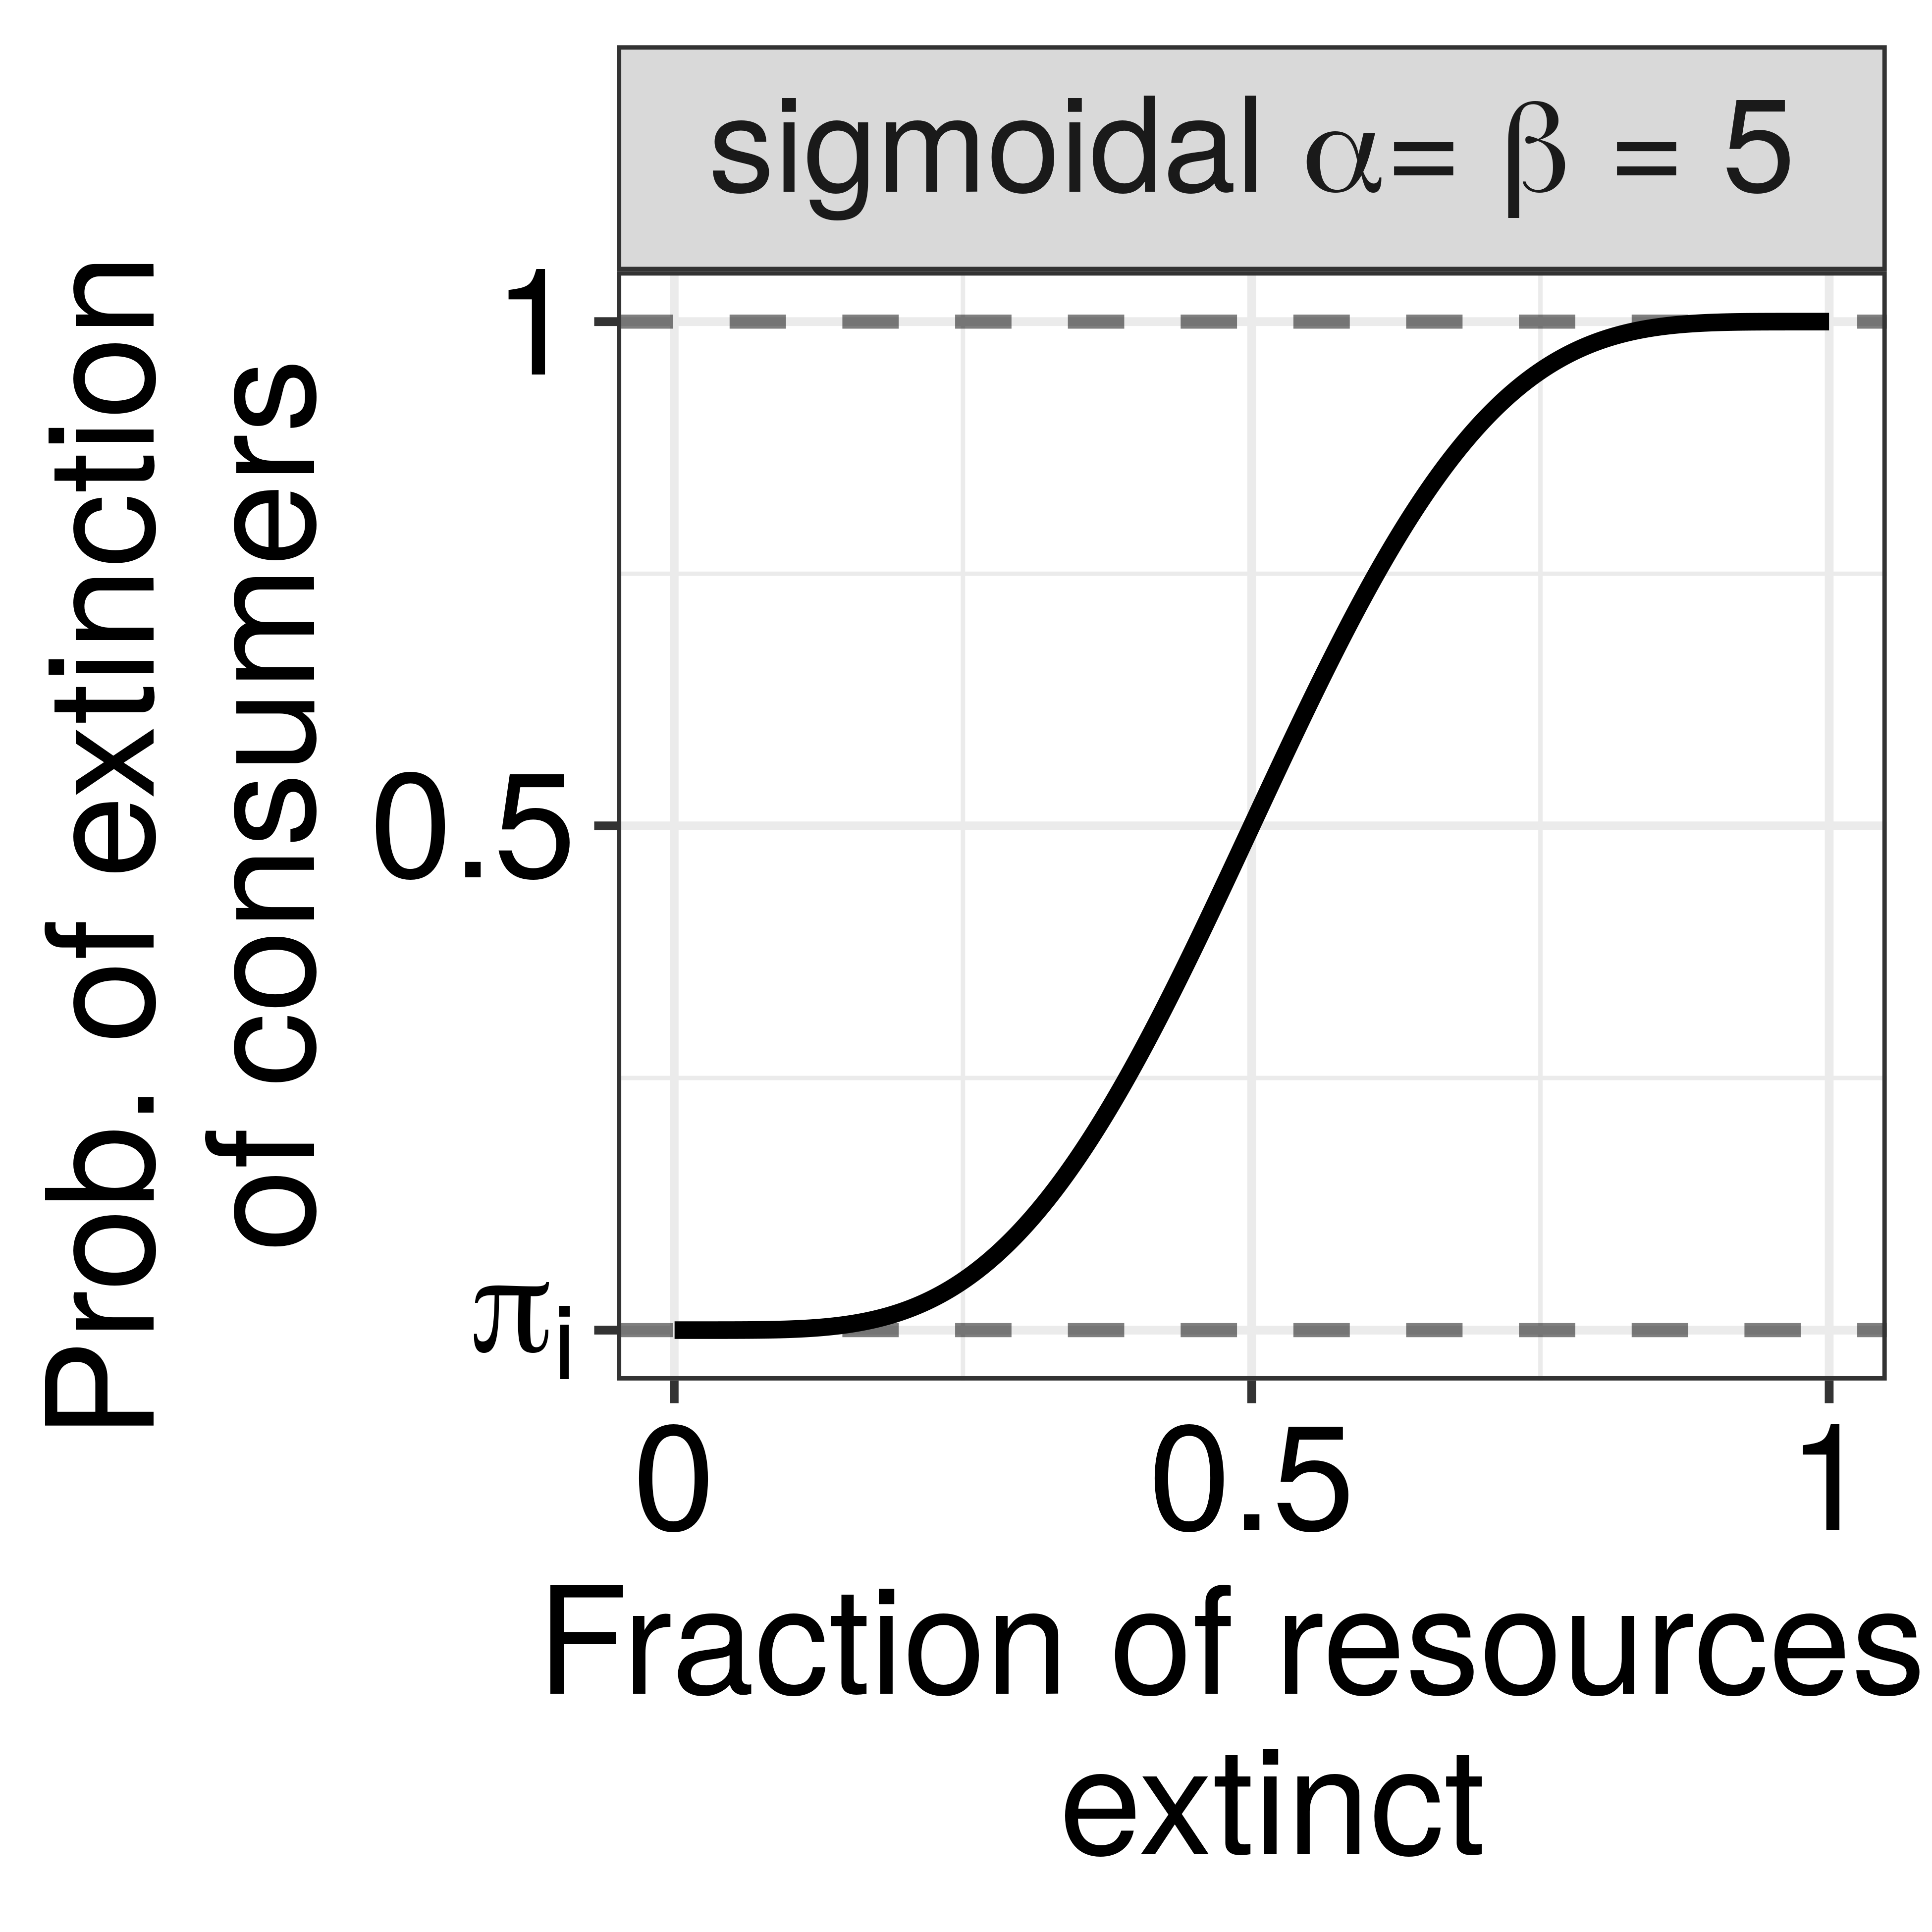
\includegraphics[width=0.18\textwidth]{fform_5_5.png}
  
\includegraphics[width=0.18\textwidth]{fform_0_0.png}
  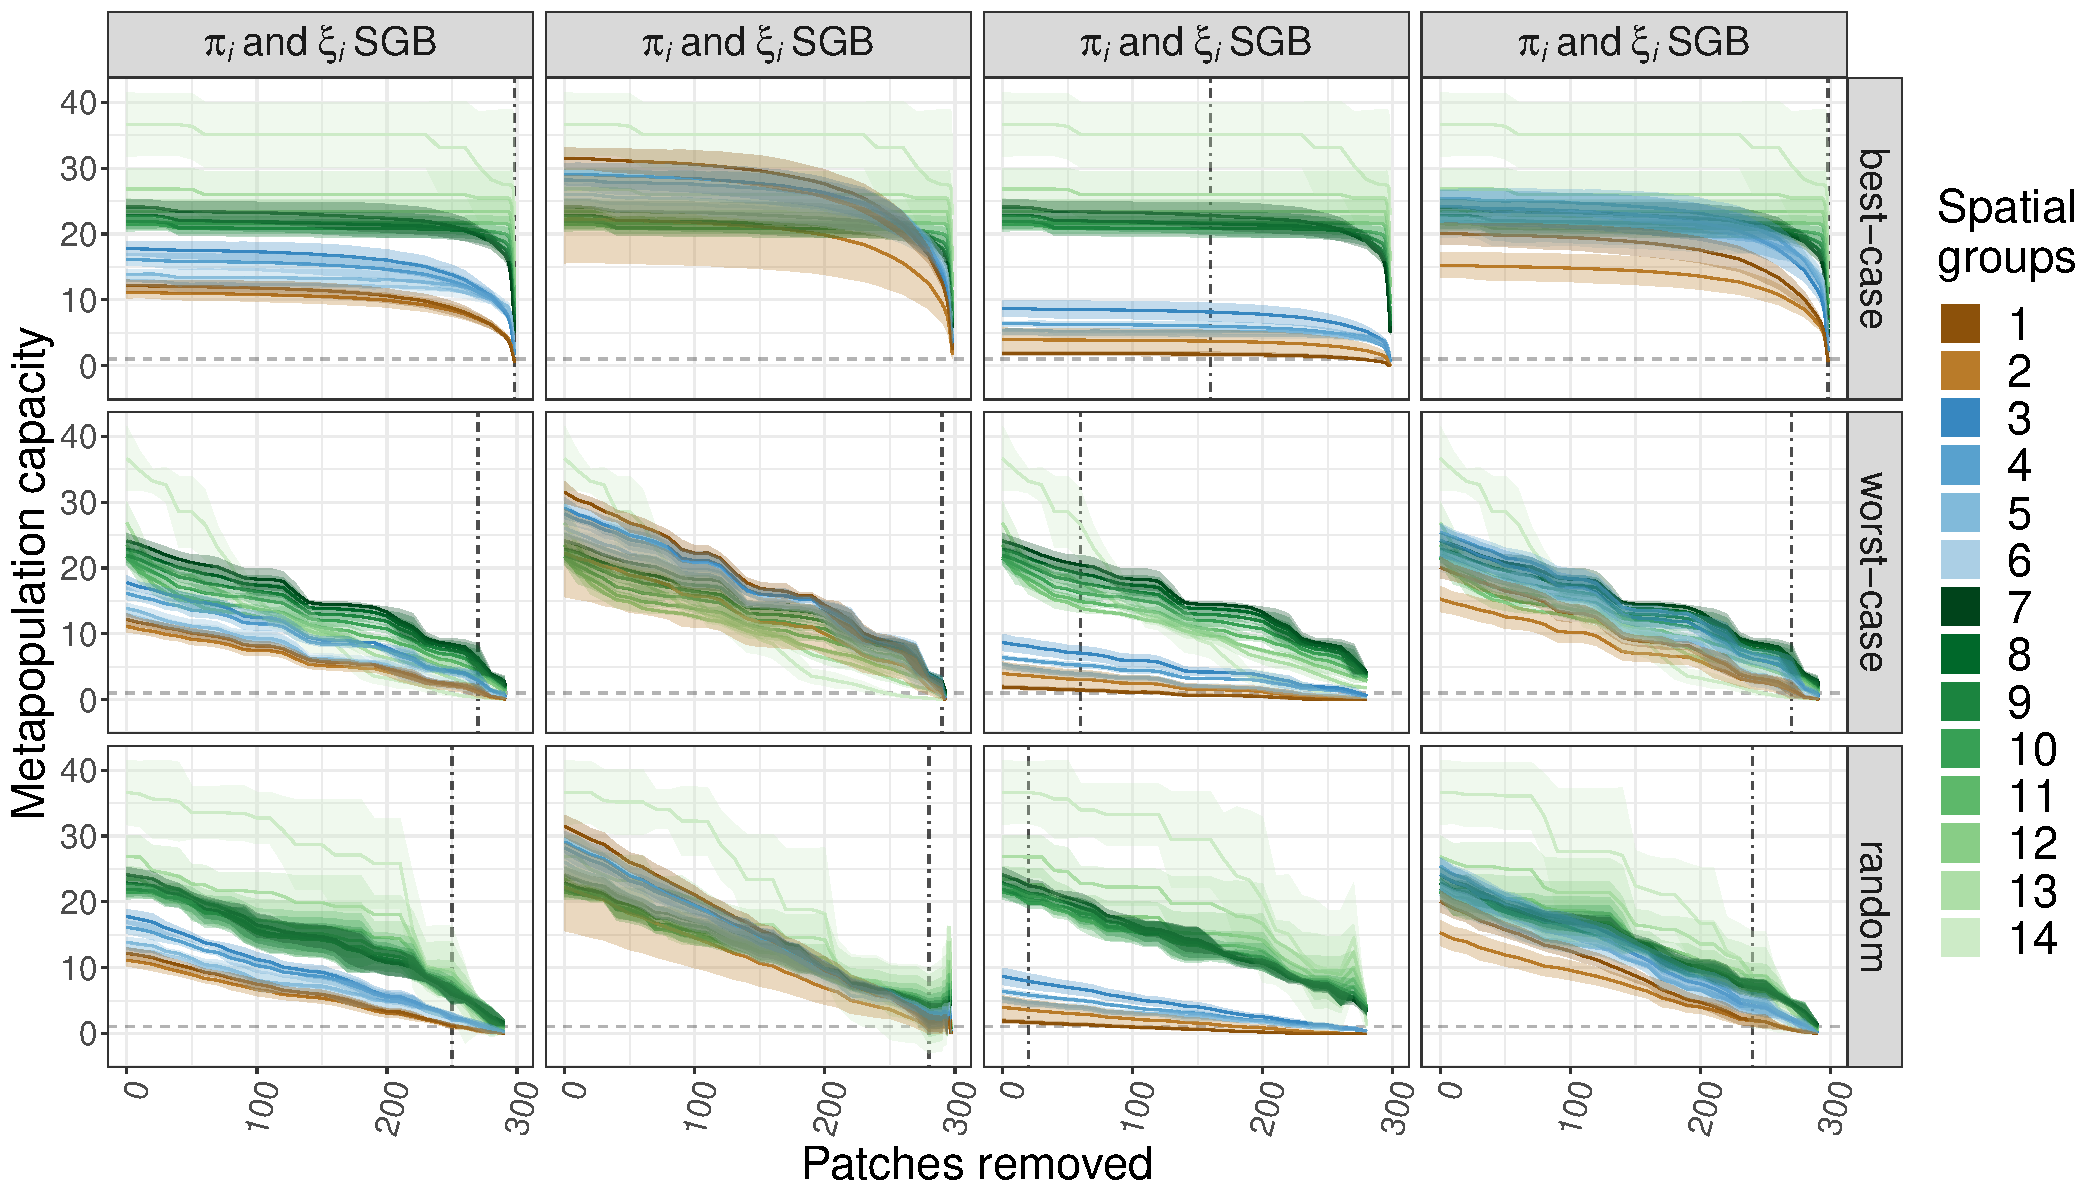
\includegraphics[width=\textwidth]{lambda_Serengeti_food_web_with_32_consumer_and_129_basal_species_basal_SGB.pdf}
  \caption{Effect of habitat loss on species persistence in the Serengeti food web. Layout as in Figure~\ref{fig:patchloss}, except color legends show spatial group instead of trophic level, and columns show different functional forms of a consumer's response to the loss of resources (top insets). We show the results for the spatial group-based parameterization (SGB), whereby both the baseline extinction probabilities $\pi_i$ and dispersal distances $\xi_i$ decrease with spatial group. In the color scheme, green colors are groups whose species are primary producers, blue colors are groups with secondary consumers, and brown colors are groups with top predators.}
  \label{fig:Serengeti}
\end{figure}


\end{document}

